 % The main file for CAMP reports
 % Don't put any content in here. 
 % Don't even include content files by using \input or \inlcude. 
 % Put your content to TEXT.TEX or include it there using \input.
 % Uses:
 %		SETTINGS.TEX	contains the settings for this document
 %		COMMANDS.TEX	contains commands which can be used while writing
 %		INFO.TEX			contains the author, title and so on for the cover
 %		COVER.TEX			formats the front cover of the document
 %		ABSTRACT.TEX	contains the abstract to be included (if needed)
 %		TEXT.TEX			contains the actual content of the document
 %		BIB.BIB				containt the BibTeX entries for the document
 
 
%% Draft document mode
%% Final document
%\documentclass[12pt,a4paper,bibtotoc,idxtotoc,headsepline,footsepline,footexclude,BCOR12mm,DIV13]{scrbook}

\documentclass[12pt,a4paper,bibtotoc,idxtotoc,headsepline,footsepline,footexclude,BCOR12mm,DIV11]{scrbook}

% KOMA-Optionen:
%  bibtotoc: include bibliography in table of contents
%  idxtotoc: include index in table of contents
%  headsepline: use horizontalline under heading
%  BCOR: binding correcion (Bindungskorrektur) (e.g.: BCOR5mm)
%  DIV: Number of sheet sections (used for layout) (e.g.: DIV12) 

% include title and author information for the cover
 % Set here the title, authors and other stuff to be used for the cover
% This file is used by MAIN.TEX

% set title, authors and stuff for the cover
\def\doctype{Bachelorarbeit in Bioinformatik}
\def\title{Feature and Label Selection in Multi-Label Classification}
\def\titleGer{Gemeinsame Feature- und Labelauswahl für Multi-Label Klassifikation}
\def\author{Sebastian Lehnerer}
\def\date{Oktober 15, 2011}

% text to appear in the footer
\def\footertext{}

% include settings
% Included by MAIN.TEX
% Defines the settings for the CAMP report document

\renewcommand{\sectfont}{\normalfont \bfseries}        % Schriftart der Kopfzeile

% manipulate footer
\usepackage{scrpage2}
\pagestyle{scrheadings}
\ifoot[\footertext]{\footertext} % \footertext set in INFO.TEX
%\setkomafont{pagehead}{\normalfont\rmfamily}
\setkomafont{pagenumber}{\normalfont\rmfamily}

%% allow sophisticated control structures
\usepackage{ifthen}

% use Palatino as default font
\usepackage{palatino}

% enable special PostScript fonts
\usepackage{pifont}

% make thumbnails
\usepackage{thumbpdf}

%to use the subfigures
\usepackage{subfigure}

\usepackage{pdfpages}
\usepackage{colortbl}
\usepackage{booktabs}

\usepackage[chapter]{algorithm}
\usepackage{algorithmic}

\usepackage[small]{caption}

%% show program code\ldots
%\usepackage{verbatim}
%\usepackage{program}

%% enable TUM symbols on title page
\usepackage{styles/tumlogo}


\usepackage{multirow}

%% use colors
\usepackage{color}

%% make fancy math
\usepackage{amsmath}
\usepackage{amsthm}
\usepackage{amsfonts}
\usepackage{amssymb}
\usepackage{textcomp}
\usepackage{yhmath} % f�r die adots 
%% mark text as preliminary
%\usepackage[draft,german,scrtime]{prelim2e}


%% create an index
\usepackage{makeidx}

% for the program environment
\usepackage{float}

%% load german babel package for german abstract
%\usepackage[german,american]{babel}
\usepackage[german,english]{babel}
\selectlanguage{english}

% use german characters as well
\usepackage[latin1]{inputenc}       % allow Latin1 characters

% use initals dropped caps - doesn't work with PDF
\usepackage{lettrine}


\usepackage{styles/shortoverview}
%----------------------------------------------------
%      Graphics and Hyperlinks
%----------------------------------------------------

%% check for pdfTeX
\ifx\pdftexversion\undefined
 %% use PostScript graphics
 \usepackage[dvips]{graphicx}
 \DeclareGraphicsExtensions{.eps,.epsi}
 \graphicspath{{figures/}{figures/review}} 
 %% allow rotations
 \usepackage{rotating}
 %% mark pages as draft copies
 %\usepackage[english,all,light]{draftcopy}
 %% use hypertex version of hyperref
 \usepackage[hypertex,hyperindex=false,colorlinks=false]{hyperref}
\else %% reduce output size \pdfcompresslevel=9
 %% declare pdfinfo
 %\pdfinfo { 
 %  /Title (my title) 
 %  /Creator (pdfLaTeX) 
 %  /Author (my name) 
 %  /Subject (my subject	) 
 %  /Keywords (my keywords)
 %}
 %% use pdf or jpg graphics
 \usepackage{graphicx}
 \DeclareGraphicsExtensions{.jpg,.JPG,.png,.pdf,.eps}
 \graphicspath{{figures/}} 

 
 %% Load float package, for enabling floating extensions
 \usepackage{float}
 
 %% allow rotations
 \usepackage{rotating}
 %% use pdftex version of hyperref
 \usepackage[pdftex,colorlinks=true,linkcolor=black,citecolor=red,%
 anchorcolor=red,bookmarks=true,%
 bookmarksopen=true,urlcolor=red,bookmarksopenlevel=0,plainpages=false%
 bookmarksnumbered=true,hyperindex=false,pdfstartview=%
 ]{hyperref}
%
%\usepackage[pdftex,colorlinks=false,linkcolor=red,citecolor=red,%
% anchorcolor=red,urlcolor=red,bookmarks=true,%
% bookmarksopen=true,bookmarksopenlevel=0,plainpages=false%
% bookmarksnumbered=true,hyperindex=false,pdfstartview=%
% ]{hyperref}
\fi




%% Fancy chapters
%\usepackage[Lenny]{fncychap}
%\usepackage[Glenn]{fncychap}
%\usepackage[Bjarne]{fncychap}

%\usepackage[avantgarde]{quotchap}

% set the bibliography style
\bibliographystyle{styles/bauermaNum}
%\bibliographystyle{alpha}
%\bibliographystyle{plain}

\sloppy

% include commands
% Commands to be used within the TUM report document
% Included by MAIN.TEX
% Please include your own cool commands here. 
% Be only sure to comment it sufficiently so others can use it.

%-------------------------------------------------------------
%                      Own Commands
%-------------------------------------------------------------


%-------------------------------------------------------------
% math stuff -------------------------------------------------

% nice R, N, C
\newcommand{\nat}{\mathbb{N}}
\newcommand{\real}{\mathbb{R}}
\newcommand{\compl}{\mathbb{C}}



% norm
\newcommand{\norm}[1]{\left\| #1 \right\|}

% un demi
\newcommand{\half}{\frac{1}{2}}

% parantheses
\newcommand{\parenth}[1]{ \left( #1 \right) }
\newcommand{\bracket}[1]{ \left[ #1 \right] }
\newcommand{\accolade}[1]{ \left\{ #1 \right\} }
%\newcommand{\angle}[1]{ \left\langle  #1 \right\rangle }

% partial derivative: %#1 function, #2 which variable
% simple / single line version
\newcommand{\pardevS}[2]{ \delta_{#1} f(#2) }
% fraction version
\newcommand{\pardevF}[2]{ \frac{\partial #1}{\partial #2} }

% render vectors: 3 and 4 dimensional
\newcommand{\veciii}[3]{\left[ \begin{array}[h]{c} #1 \\ #2 \\ #3	\end{array} \right]}
\newcommand{\veciv}[4]{\left[ \begin{array}[h]{c} #1 \\ #2 \\ #3 \\ #4	\end{array} \right]}

% render matrices: 3  dimensional (arguments in row first order)
\newcommand{\matiii}[9]{\left[ \begin{array}[h]{ccc} #1 & #2 & #3 \\ #4 & #5 & #6 \\ #7 & #8 & #9	\end{array} \right]}
%DOESN'T WORK,DON'T KNOW WHY \newcommand{\mativ}[16]{\left[ \begin{array}[h]{cccc} #1 & #2 & #3 & #4 \\ #5 & #6 & #7 & #8 \\ #9 & #10 & #11 & #12 \\ #13 & #14 & #15 & #16 \end{array} \right]}


%-------------------------------------------------------------
%-------------------------------------------------------------


%-------------------------------------------------------------
% some abreviations ------------------------------------------
\newcommand{\Reg}{$^{\textregistered}$}
\newcommand{\reg}{$^{\textregistered}$ }
\newcommand{\Tm}{\texttrademark}
\newcommand{\tm}{\texttrademark~}
\newcommand {\bsl} {$\backslash$}

%-------------------------------------------------------------
%-------------------------------------------------------------


%-------------------------------------------------------------
% formating --------------------------------------------------

% Theorem & Co environments and counters
\newtheorem{theorem}{Theorem}[chapter]
%\newtheorem{task}{Task}
\newtheorem*{task}{Task}
\newtheorem{lemma}[theorem]{Lemma}
\newtheorem{corollary}[theorem]{Corollary}
\newtheorem{remark}[theorem]{Remark}
\newtheorem{definition}[theorem]{Definition}
\newtheorem{equat}[theorem]{Equation}
\newtheorem{example}[theorem]{Example}
%\newtheorem{algorithm}[theorem]{Algorithm}

% inserting figures
\newcommand{\insertfigure}[4]{ % Filename, Caption, Label, Width percent of textwidth
	\begin{figure}[htbp]
		\begin{center}
			\includegraphics[width=#4\textwidth]{#1}
		\end{center}
		\vspace{-0.4cm}
		\caption{#2}
		\label{#3}
	\end{figure}
}




% referecing figures

\newcommand{\refFigure}[1]{ %label
	figure \ref{#1}
}
\newcommand{\refChapter}[1]{ %label
	chapter \ref{#1}
}

\newcommand{\refSection}[1]{ %label
	section \ref{#1}
}

\newcommand{\refParagraph}[1]{ %label
	paragraph \ref{#1}
}

\newcommand{\refEquation}[1]{ %label
	equation \ref{#1}
}

\newcommand{\refTable}[1]{ %label
	table \ref{#1}
}




\newcommand{\rigidTransform}[2]
{
	${}^{#2}\!\mathbf{H}_{#1}$
}

%code, in typewriter
\newcommand{\code}[1]
 {\texttt{#1}}

% comment that appears on the border - very practical !!!
\newcommand{\comment}[1]{\marginpar{\raggedright \noindent \footnotesize {\sl #1} }}

% page clearing
\newcommand{\clearemptydoublepage}{%
  \ifthenelse{\boolean{@twoside}}{\newpage{\pagestyle{empty}\cleardoublepage}}%
  {\clearpage}}


%-------------------------------------------------------------
%-------------------------------------------------------------


\newcommand{\etAl}{\emph{et al.}\mbox{ }}


%\makeindex
	%% inter line spacing
%\linespread{1.0}

\makeglossary

\begin{document}

	\frontmatter
		
	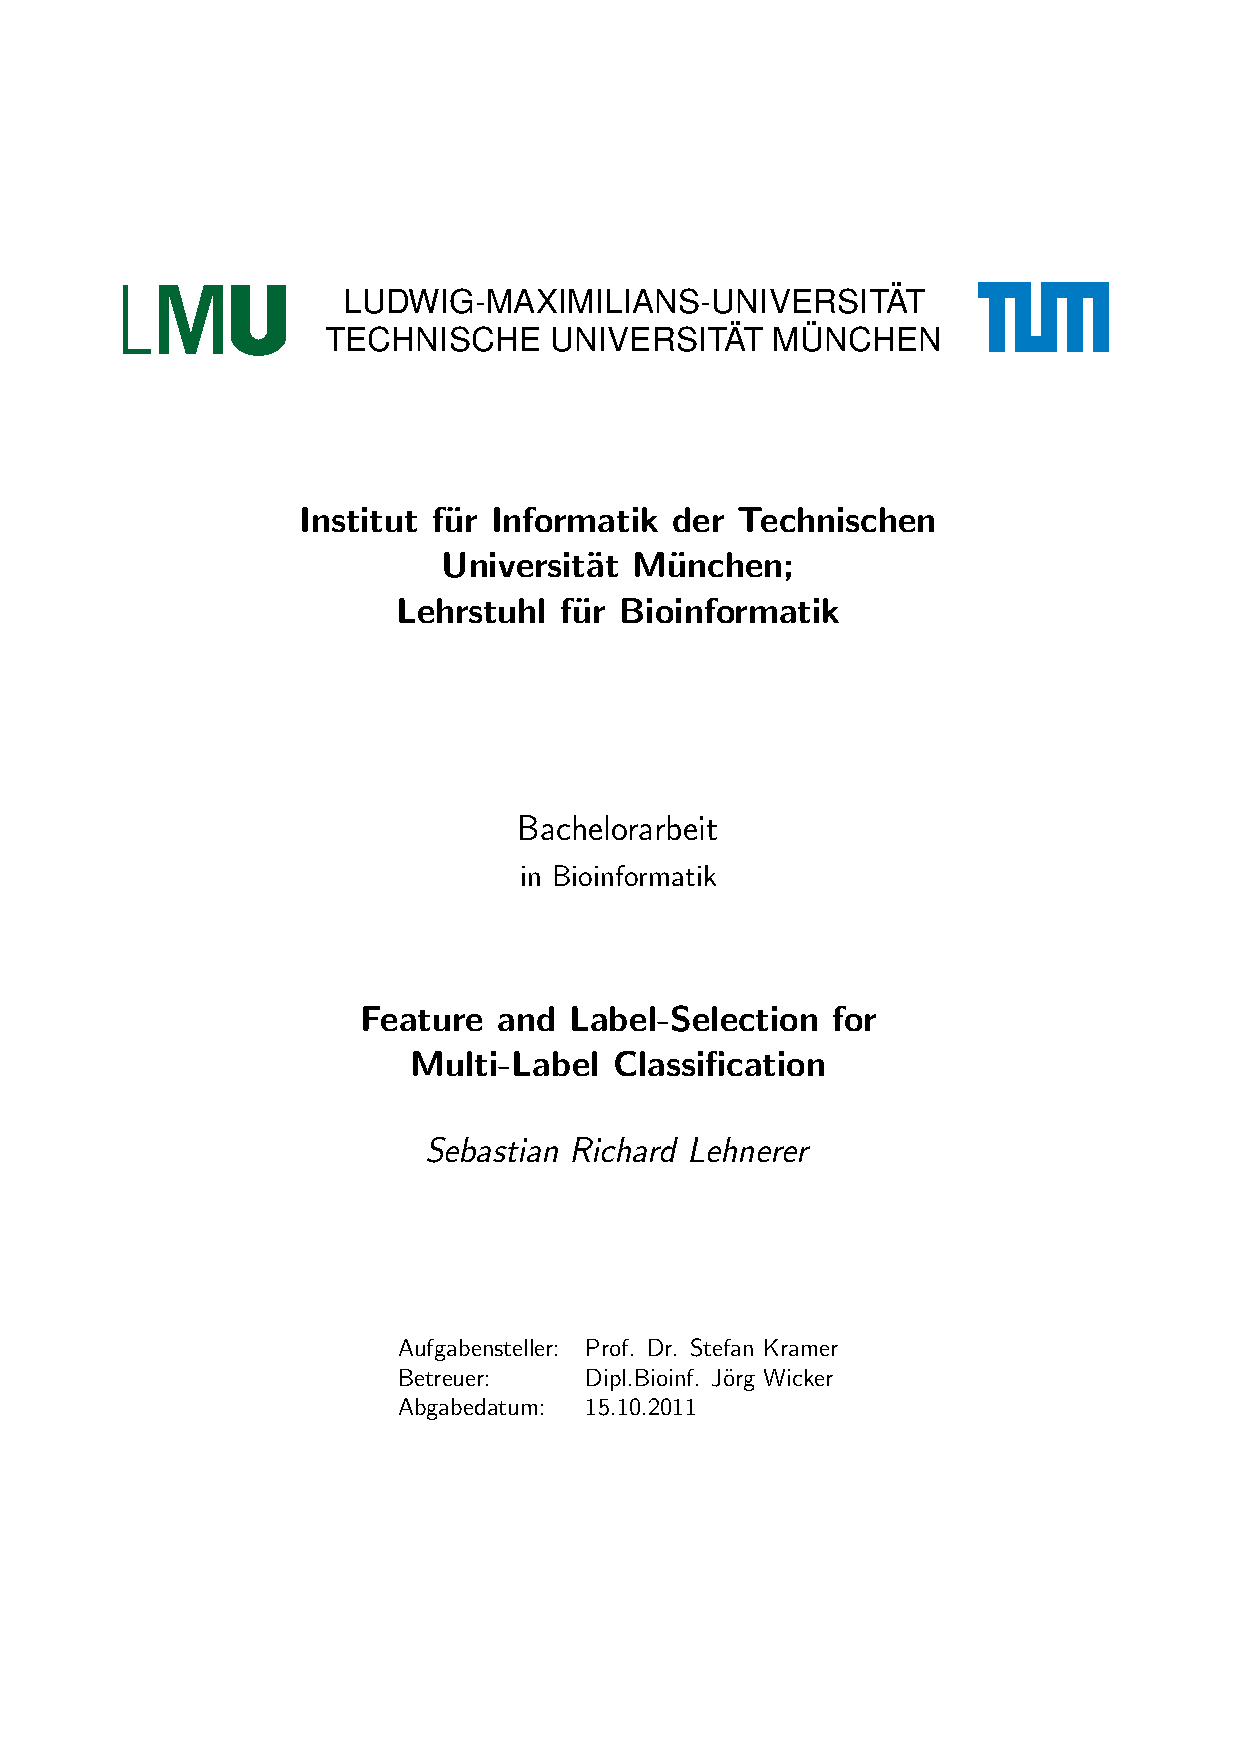
\includepdf[pages={1}]{title.pdf}
	
	\clearemptydoublepage


\thispagestyle{empty}
\selectlanguage{german}
	\vspace*{0.8\textheight}
	\noindent
	Ich versichere, dass ich diese Diplomarbeit selbst{\"a}ndig verfasst und nur 
	die angegebenen Quellen und Hilfsmittel verwendet habe.
	
	\vspace{15mm}
	\noindent
	M{\"u}nchen, den \today \hspace{4cm} \author
\selectlanguage{english}
\newpage
	
	%\clearemptydoublepage
\phantomsection
\addcontentsline{toc}{chapter}{Acknowledgements}	


%\chapter*{Acknowledgements}

\vspace*{2cm}

\begin{center}
{\Large \bf Acknowledgments}
\end{center}

\vspace{1cm}




If someone contributed to the thesis... might be good to thank them here.
	
	% Abstract for the TUM report document
% Included by MAIN.TEX


\clearemptydoublepage
\phantomsection
\addcontentsline{toc}{chapter}{Abstract}	





\vspace*{2cm}
\begin{center}
{\Large \bf Abstract}
\end{center}
\vspace{1cm}

\paragraph*{} This bachelor thesis presents a new approach for Feature and Label Selection for Multi-Label Classification. In general, classification is the task of assigning one or more labels to an unseen instance. Multi-label classification is concerned with the assignment of a set of labels is assigned to each instance. This is useful for applications such as protein function annotation and prediction of toxicological endpoints. This work bases on the assumption that there exist subsets of the label and feature space having a higher internal dependence than to the rest of data. Here, two methods are proposed to identify those groups and apply any multi-label learning scheme on it. It can be shown that splitting the dataset into subgroups does not affect the performance, yet it does yield improvements in some cases.

\paragraph*{} Diese Bachelorarbeit zeigt einen neuen Ansatz zur Feature und Label-Auswahl zur Multi-Label Klassifizierung. Allgemein beschreibt Klassifizierung die Aufgabe unbekannten Objekten eine oder mehrere Klassen zuzuordnen. Dieser Schritt wird Multi-Label Klassifizierung genannt, wenn jedem Objekt eine Menge von Klassen zugeordnet wird. Dies ist unter anderem n\"utzlich zur Protein-Funktionsanalyse sowie zur Bestimmung der Toxizit\"at unklassifizierter Substanzen. Diese Arbeit basiert auf der Annahme, dass innerhalb dieser Daten Untergruppen von Features und Labels bestehen die einen gr\"o\ss{}eren Zusammenhang aufweisen als zu den restlichen Attributen. Zwei Methoden wurden entwickelt um diese Untergruppen zu identifizieren und Multi-Label Klassifikatoren auf diesen zu lernen. Es konnte gezeigt werden, dass die Zerteilung der Feature- und Label-Menge keinen negativen Einfluss auf die Vorhersagegenauigkeit hat. In einigen F\"allen konnte sogar eine Verbesserung festgestellt werden. 

	\tableofcontents
  
  	\mainmatter
	
	% Put your content in here or include it by using \input (\include won't work)

\addtolength{\evensidemargin}{-12mm}

		\chapter{Introduction and Related Work}
\label{chapter:IntroductionAndRelatedWork}
	\section{Description of the field}
	\label{sec:description}
		Computational biology has become an essential part of modern biology, biochemistry and medicine. Closely related fields like chemoinformatics, immunoinformatics and system biology spread the tools of computational science to many fields of life science. Bioinformatics or computational biology aims to collect, categorize, store and analyze biological systems \cite{Luscombe01}: Some time before the Human Genome Project \cite{human01} biologists became aware of the powerful possibilities of computational science. Successively a huge amount of data, e.g. gene sequences, structural information, interactions and other, data was collected. In the beginning, bioinformatics enabled the storage of those data in databases like SWISSPROT \cite{Bairoch:1996} and the Protein Data Bank (PDB)\footnote{\url{http://www.rcsb.org/pdb/}}. After storing and cataloging data, analyzing steps to discover patterns and structures within the data \cite{Luscombe01} were developed.

		Knowledge discovery in databases (KDD) \cite{Fayyad96fromdata} processes large datasets and aims to discover patterns within the data using statistical methods as well methods from artificial intelligence. It offers deep insight into the data and a better understanding of the underlying  patterns. The process of mining patterns describing the data is called descriptive data mining. On the other hand, predictive data mining allows extracting models and offers methods to classify unseen examples.
		
		Unsupervised learning is the task to find patterns like clusters in unlabeled data. Supervised learning refers to the task of learning models to classify labeled data. It maps an instance of features to an output variable called label. Supervised learning can be split into classification and regression analysis. While classification predicts discrete values, regression analysis offers methods to predict continuous target variables. Besides clustering and association rule learning, classification is one of the core areas in data mining. 

		Classification is the process of assigning categories to examples of data \cite{mitchell97}. A common example is the \textit{PlayTennis}-Problem whether to play tennis or not. Given a dataset which maps features like weather or weekday to the decision play tennis or not, the goal is to learn a model predicting this target value using the given features. An example is shown in table \ref{tab:tennis}.

			\begin{table}
				\begin{center}
					\begin{tabular}{|c|c|c|}
						\hline
						weather & weekday & class \\ 
						\hline \hline 
						sunny & Sunday & yes \\ 
						\hline 
						sunny & Monday & no \\ 
						\hline 
						rain & Sunday & no \\ 
						\hline 
					\end{tabular}
				\caption{Example for classification: Columns describe features, the last column represents the class. The class corresponds to the decision if the user plays tennis or not. Examples are showed in rows.\\ If the tennis court is only available on weekends and the user only plays tennis on sunny days only the first instance will be classified to $yes$, both other instance will be classified to $no$. } 
				\label{tab:tennis}
			\end{center}
		\end{table}

		Amongst others, there are two basic extensions of the task of classification: 1) from a binary to a multi-class classification problem, where more than two categories are available and 2) to a multi-label problem. The latter one is given if an instance is associated with a set of categories (labels) \cite{Tsoumakas07}.

			\paragraph{Definition}
				Formally, a dataset $D$ can be described as follows: \mbox{$ D= \{(x_i,Y_i) | i=1...|D|\} $}, where each instance $(x_i,Y_i)$ consists of a feature vector $x_i$ and a subset of labels/classes $Y_i\subseteq L$, where $L$ is the full set of labels. Single-label classification is concerned if a class $ \lambda \in L $ is assigned to instances. Binary classification refers to label sets $L$ of cardinality 2 ($|L|=2$), multi-class classification to sets $ |L|>2 $. In both cases classifiers choose out of $|L|$ classes but always only one class $\lambda$ is assigned to an instance. In multi-label classification, a subset $ Y\subseteq L $ is assigned to each instance, therefore a classifier has to choose a set of assigned labels as well as the number of assigned labels. Another aspect of multi-label classification is to produce a ranking of labels along to its relevance to the current example.

			\paragraph{Applications}
				For instance, pictures mostly match not only one category, but show a combination of different categories like hill, forest, water or beach. Another example would be movies like \textit{Da Vinci Code} which can be categorized as Society\textbackslash Religion and Arts\textbackslash Movies \cite{Tsoumakas07}.

				An application in bioinformatics for multi-label classification is the ToxCast\tm project \cite{Dix07}. The project started in 2007. 320 different chemical structures were tested for toxicological endpoints. About 1600 properties and more than 400 endpoints were examined.

				The goal of this project is to map \textit{in vitro} measured features to \textit{in vivo} observed toxicological endpoints, which is a classic task of classification. Particularly, it is a challenging task for multi-label learning, as the set of toxicological endpoints (400), which refer to labels and the set of features (1600), is quite large. Once this is done, predictions about the toxicity of chemical substances/structures can be made without tedious lab-work or morally questionable animal experiments.

	\section{Motivation}
		\begin{task}
			For a dataset \mbox{$ D= \{(x_i,Y_i) | i=1...|D|\} $} with a feature vector $ x_i $, label set \mbox{$ Y_i \subseteq L$}, there exists a subset \mbox{$ L_G \subseteq L $} of all labels and a corresponding subset \mbox{$ X_G \subseteq X $} of features forming a subset of the data \mbox{$ G \subseteq D $} with \mbox{$ G = \{({x_G}_i,{Y_G}_i) | i=1...|G|\} $}, in which attributes have a high internal association.
		\label{theorem}
		\end{task}

		In many multi-label applications there exist groups of connected labels and features which come naturally. E.g. in the picture labeling example, it is probable to see combinations of water, beach and island. On the other hand, it is very improbable to see combinations like forests and desert. Another example would be the ToxCast\tm dataset, where it is highly probable to find families of in vitro features connected to a group of similar in vivo endpoints. Therefore, there will be specific features for specific labels. For instance, the blue content of a picture may be important for the label \textit{sea} and \textit{sky}, but irrelevant to other labels like \textit{forests}.

		Based on this assumption, this work aims to develop a method to find sets of labels and corresponding features. Subsequently, multi-label learners can be applied on those sub-datasets. Experiments show that those models achieve better performance in some cases since they can fit to characteristic groups. In addition, subsets representing independent information patterns can be isolated.

		The bachelor thesis is organized as follows: Firstly core components like clustering and feature selection are described. Subsequently, two Feature- and Label-Selection for Multi-Label Classification methods are presented in this work. Finally, it concludes with a presentation of the evaluation and discussion of benefits of these methods.

	\section{Related Work}
	\label{sec:relatedwork}

		This chapter gives an overview on existing multi-label classification techniques. HOMER is described here, as it uses a similar approach to this work, despite its focus lies on efficiency rather than structural decomposition. 
		
		\paragraph{Notation} The following notation is used for describing the multi-label problems: $ D $ is the dataset composed of n examples $ (x_1,Y_1), (x_2,Y_2), \hdots, (x_n,Y_n) $, where $ x_i $ is the instance containing the feature values and $ Y_i \subseteq L $ a subset of labels associated with this instance. A vector $\vec{y_i} = [y_{i_1}\hdots y_{i_L}] = \{0,1\}^L$ is used to describe $Y_i$, where $\vec{y_{i_j}}=1$ if the $j$th label is relevant (otherwise  $\vec{y_{i_j}}=0$). Single labels are annotated with $\lambda_{1\hdots L}$.

			\subsection{Multi-Label Classification Methods}
			\label{subsec:mlmethods}
				There are two groups of multi-label classification methods \cite{Tsoumakas07}:
				\begin{enumerate}
					\item Transformation-based methods, which transform the problem in to several single-label problems and apply binary classification methods (e.g. SVMs \cite{SVM}, Decision Trees \cite{Quinlan1986}, k-Nearest-Neighbors \cite{mitchell97}). An exception is the Label Powerset method, which transforms the problem to a multi-class classification task. 
					\item Algorithm-adaptation methods, which extend existing algorithms to be capable of handling multi-label problems directly.
				\end{enumerate}
				
				\subsubsection{Transformation based Methods}
				\label{subsubsec:transformation}
					\paragraph{Binary Relevance}
					\label{para:br}
						A basic multi-label classification method is Binary Relevance (BR) \cite{Tsoumakas07}. This method transforms the multi-label problem into $ |L| $ separate problems and trains a single-label learner on each on them. The prediction is simply composed by the prediction of the single classifications $ \lambda_1\hdots \lambda_n $. It does not take any dependencies between labels into account. This makes it the simplest multi-label learner. Labels tend to have strong inter-relationships, however, BR does not consider those relationships, thus predictions on a label $ l_i $ have no influence on predictions of other labels $ l_j $. However, it is still popular as it scales linear with the number of labels, thus complexity lies in $ O(|L|) $.
						
					\paragraph{Label Powerset}
					\label{para:lp}
						The Label Powerset method includes label dependencies but suffers from computational complexity. For every unique set $ Y $ of labels in the data, a class $ l_Y $ is created, representing this combination. Subsequently, and a multi-class classifier is built on the data. Thus, every combination is represented as a single class and label correlations are taken into account directly. Despite the worst-time complexity of $ O(2^{|L|}) $ another disadvantage is that, in its basic form, it can only predict label combinations which are present in the training data.
					
					\paragraph{Multi-Label Stacking}
					\label{para:ms}
						Multi-label Stacking or $ BR^2 $ deals with the disadvantage of BR by not taking label relations into account \cite{Tsoumakas09}. Therefore, a stacking mechanism is used. The first level of Multi-label Stacking consists of a BR classifier predicting labels independently. A second level incorporates the output of the first level BR classifier, in detail the label confidences. Result is a relation-dependent prediction.	Formally, first step produces a dataset \mbox{$ D'=\{(y_i,Y_i),i=1\hdots |D|)\}$}. The vector $ y_i $ contains all predicted confidences of the base level for all labels $\lambda_{1\hdots |D|}$ of an instance $ i $. Subsequently, for every label a meta level binary classifier is used to classify, resulting in a prediction of $\lambda_{1\hdots |D|}$. To reduce the noise, $\phi$ correlations between all labels in the original data is computed. For the meta level, only labels exceeding the correlation threshold are used. By this, the dimensionality of the feature space in the meta-level and also the noise will be reduced.

					\paragraph{Classifier Chains}
					\label{para:cc}
						Classifier Chains by Read \etAl \cite{Read09} handles the label correlations by using a chain of single-label classifiers. Each of them is predicting the labels subsequently, e.g. for every label $ \lambda $ in the label set $ L $ a single-label classifier $C_{1\hdots |D|}$ is trained. Every member in the chain adds feature with the confidence of the prediction for the current label to the feature space. Thus every classifier can use the prediction of the previous labels. The order of the chain influences the performance, nevertheless current implementations are using a random order. The performance can be improved by using ensembles of randomly ordered Classifier Chains.

				\subsubsection{Algorithm-adoption methods}
				\label{subsubsec:adaption}
					\paragraph{ML-kNN}
					\label{para:mlknn}
						ML-kNN proposed by Min-Ling Zhang and Zhi-Hua Zhou \cite{Zhang05} is an adaption of the k-Nearest-Neighbor algorithm. As first step the $k$ nearest neighbors are calculated, subsequently the label sets are mapped using the maximum-a-posteriori principle (MAP) based on the information gain about the label sets of the neighboring instances. The method is described in more detail in algorithm \ref{algo:mlknn}. Given a dataset \mbox{$ D'=\{(y_i,Y_i),i=1\hdots |D|)\}$} and label set $ L=\lambda_{1\hdots|D|}$, a \textit{membership counting} vector $ \vec{C}_I(l) $ is used representing the number of neighbors of instance $ I $ which are associated with label $\lambda$. $ N(I) $ is the set of the $k$ nearest neighbors of instance $I$. $H^\lambda_1$ is the event that $t$ is associated with label $\lambda$ in contrast $H^\lambda_0$ is the event that $I$ is not associated with label $\lambda$. With $E^\lambda_j:j=0..k$ the event that among the $k$ nearest neighbors are exactly $j$ instances labeled with label $\lambda$.
With those variables for each instance $i$ a \textit{category vector} $\vec{y}_I(\lambda)$ can be computed where $ \vec{y}_I(\lambda) $ is 1 if $ \lambda $ is among the predicted label set $Y_{I_{pred}} $ for instance $I$. The vector $\vec{r}_I(\lambda)$ is holding numeric values to generate a ordering of the labels in order to predict a ranking instead a fixed label set.

						\begin{algorithm}
							\begin{algorithmic}
								\REQUIRE $ I = (x_i,Y_i) \in D $  \COMMENT{input is an instance \ensuremath{I}}
								\STATE Identify $N(I)$ \COMMENT{identify the \ensuremath{k} nearest neighbors}
								\FOR[compute for every label:]{$ \lambda \in L $}
									\STATE $\vec{C}_I(\lambda)=\sum_{a\in N(I)}\vec{y}_{x_a}(\lambda)$ \COMMENT{membership vector}
									\STATE $\vec{y}_I(\lambda)=\arg\max_{b\in \{0,1\}} P(H^\lambda_b)P(E^\lambda_{\vec{C}_I(\lambda)}|H^\lambda_b)$ \COMMENT{category vector}
									\STATE $\vec{r}_I(\lambda)=P(E^\lambda_{\vec{C}_I(\lambda)}|H^\lambda_b)$ \COMMENT{category vector with real values for ranking}
								\ENDFOR
								\RETURN $\vec{y}_I$ and $\vec{r}_I$
							\end{algorithmic}
							\caption{ML-kNN} 
							\label{algo:mlknn}
						\end{algorithm}

				\subsubsection{HOMER}
				\label{subsubsec:homer}					
					A multi-label learner introduced by Tsoumakas \etAl \cite{Tsoumakas08} called HOMER is based upon a Hierarchy Of Multilabel classifERs. In order to build the hierarchy the label set $L$ is split into $k$ disjoint subsets. This is done recursively for each subset, until the number of remaining labels is $<k$. For every step in the hierarchy, clustering is used to find $k$ clusters of similar labels. To ensure a balanced label distribution for each cluster, a modified cluster algorithm based on k-means, called \textit{balanced k-means}, is used. For the clustering only the label part of data is used. The result is a tree-like hierarchy of $L$ with $L_{root}=L$ and every single label as leaf. A meta-label level rules the path through the hierarchy. An instance $ I $ is annotated with meta-label $\mu_n$ if it is associated with any label of $L_n$. For every internal node, a classifier is trained, predicting current meta-label $\mu_n$. Therefore, only branches with positive meta-labels will be considered for multi-label predicting, reducing the computational costs, because for every branch a classifier has to deal with a much smaller label set. As classifiers have to deal with a much smaller set of labels in each level and only those branches with positive meta-labels are evaluated, a linear training and predicting complexity of $O(log_k(|L|))$ can be achieved.
		\clearemptydoublepage		
		
		\chapter{Clustering and Feature Selection}
\label{chap:clusteringandfeatureselection}

	Clustering and feature selection methods are core elements of this work. Thus, this chapter gives an introduction to the field and an overview over the used clustering and feature selection methods.

	\section{Cluster analysis}
	\label{sec:clustering}

		Cluster analysis or clustering is the task of assigning instances to subsets called clusters which are most similar inside and most dissimilar outside the cluster in respect to some distance or similarity measure. Clustering is an unsupervised method and does not use class information.

		An application for clustering is gene expression analysis. Clustering methods are used to identify groups of genes with higher expression, than other groups. In line with the experiment, one can find families of genes which are correlated, and map co-expressions to diseases or biological pathways.

		Many cluster methods require specifying the number of clusters prior to the process of clustering. This requires knowledge of the underlying structure of the dataset which is often not available or even the goal of the experiment. Cluster methods assign every instance to one particular cluster. However some cluster methods like Expectation Maximization (EM) compute membership probabilities. This is used to create a non-deterministic clustering of the data, allowing assigning cluster instances according to its membership probability.

		There exists methods to evaluate a clustering. One of the most intuitive ones is to assign a class to each instance, separating the desired groups of instances. An optimal cluster method discriminates classes in different clusters. In this work, clustering is evaluated with respect to label dimensions, as density, cardinality and correlation as well to classification evaluation measures like accuracy.

		Clustering will be used in order to find groups of correlated labels in multi-label datasets. Three types of clustering methods have been used.

		\subsection{Clustering Methods}
		\label{subsec:clustering}
			\subsubsection{Hierarchical Clustering}
			\label{subsubsec:hirach}
				
				Hierarchical Clustering creates a hierarchy of clusters, either starting from one cluster and splitting, until every instance is its own cluster, called top-down or divisive clustering, or starting with every instance in a separate cluster and merging until all instances remain in one cluster, named bottom-up or agglomerative clustering \cite{Jain99}.

				Agglomerative clustering has a lower computational complexity as divisive clustering because splitting criteria can be computed directly, where most merging criteria need some "look-ahead" procedure. 

				Agglomerative clustering consists of three steps:
				
				\begin{enumerate} 
					\item{Compute a proximity matrix in-between each pair of clusters.}
					\item{Merge the closest clusters.}
					\item{Go to Step 1 until a minimum number of clusters are reached, or all instances remain in one cluster}
				\end{enumerate}

				\paragraph{Linkage criteria}
					The linkage criteria describes how the distance between clusters is computed. In the following, the linkage criteria used in this work are presented.

					\begin{enumerate}
						\item{Single linkage is the minimum distance between two clusters \mbox{A and B}
						\begin{equation}
							\min \, \{\, d(a,b) : a \in A,\, b \in B \,\}
						\end{equation}}
						
						\item{Complete linkage is the maximum distance between two clusters 	\mbox{A and B}
						\begin{equation}
							\max \, \{\, d(a,b) : a \in A,\, b \in B \,\}
						\end{equation}}
	
						\item{Average linkage is the mean distance of all elements in clusters \mbox{A and B}
						\begin{equation}
							\tfrac{1}{|A||B|}\sum_{a\in A, b\in B} d(a,b)
						\end{equation}}
						
						\item{Average group linkage is the mean distance of all elements in the junction of clusters \mbox{A and B} (also called Mean Linkage)
						\begin{equation}
							\tfrac{1}{(|A|+|B|)(|A|+|B|-1)}\sum_{x,y\in A \cup B} d(x,y)
						\end{equation}}
					\end{enumerate}

					\paragraph{Measures}
					\label{para:measures}
					
						For computing the proximity, any metric can be used. Fundamental ones are the Euclidean and Manhattan-Distance (also Taxicab-Distance):

						\begin{eqnarray}
							D_{\rm Euclidean}(x_i,x_j) :=\sqrt{\sum_{k=1}^p (x_{ik}-x_{jk})^2} \label{eqn:euclidean}\\
							D_{\rm Manhatten}(x_i,x_j) :=\sum_{k=1}^p |x_{ik}-x_{jk}|				\label{eqn:manhatten}
						\end{eqnarray}

						Note: $p$ is the length of the vector $x$.
						
						The Chebyshev-Distance as the maximum distance of its elements:

						\begin{equation}
							D_{\rm Chebyshev}(x_i,x_j) := \max_k^p(|x_{ik} - x_{jk}|)
						\end{equation}

%In this work also the Tanimoto Distance \cite{Tanimoto60} is used. The Tanimoto Distance is an application on binary data, i.e. on sets where objects can be contained or not. It is calculated using the similarity ratio
%
%\begin{equation}
%T_s(x_i,x_j) =  \frac{\sum_k^p ( x_{ik} \land x_{jk})}{\sum_k^p ( x_{ik} \lor x_{jk}))}
%\end{equation}
%
%and a distance measure
%
%\begin{equation}
%D_{Tanimoto}(x_i,x_j) = -{\log} _2 ( T_s(x_i,x_j) ) 
%\end{equation}

						Some feature selection methods produce a ranking of features. To apply hierarchical clustering on ranked features the Spearman Rank Correlation Coefficient \cite{Myers03} is used:

						\begin{equation}
							\rho = \frac{\sum_i(x_i-\bar{x})(y_i-\bar{y})}{\sqrt{\sum_i (x_i-\bar{x})^2 \sum_i(y_i-\bar{y})^2}}
						\end{equation}

						Note $x_i$,$y_i$ are ranks, $\bar{x}$, $\bar{y}$ is the mean rank of x, respective y.
											
						As there will occur no ties\footnote{multiple elements sharing the same rank}, in this application, a simpler formula introduced by Myers \textit{et. al} can be used \cite{Myers03}:
						\begin{equation}
							\rho = 1- {\frac {6 \sum d_i^2}{n(n^2 - 1)}}
						\end{equation}
	
						where $ d_i $ is the difference between the ranks $ d_i = x_i - y_i $ and $ n $ the number of examples.

						Divisive clustering methods like DIANA \cite{Kaufman90} generally have higher computational complexity, thus they are not included in this work. Future work may explore more cluster methods as well as divisive clustering.

					\subsubsection{k-means Clustering}
					\label{subsubsec:kmeans}

						k-Means is another clustering algorithm based on distance metrics \cite{MacQueen67}. k-Means assigns examples to one of $ k $ clusters, as shown in algorithm \ref{algo:kmeans}.

						\begin{algorithm}
							\caption{k-means clustering}
							\label{algo:kmeans}
							\begin{algorithmic}
								\STATE init $c_{1..k}$ as cluster centers randomly
								\WHILE{repeat $ < n $ OR $c_{1..k}$ converge}
									\STATE (2) assign each example $ x $ to the nearest cluster ($ \min_{i} (d(c_i,x))$), where $d(x,y)$ is any metric
									\STATE (3) recompute $c_{1..k}$ as the geometric centroid for each cluster
								\ENDWHILE
							\end{algorithmic}
						\end{algorithm}

						After a randomly initialization of $k$ cluster centers, each instance is  assigned to its nearest cluster according to a distance measure. After assigning the instances the cluster center is recomputed. Step 2 \& 3 is repeated at a most $ n $ times or until the center positions converge. To compute the distance $ d(c_i,x) $ one can use any metric. It is faster than the Hierarchical Clustering as it does not need to update a full $n\times n$ distance matrix, but only the distance to the cluster center $ c_i $. However, k-means converges to a local optimum. Solutions can still be improved by re-starts.

					\subsubsection{Expectation Maximization}
					\label{subsubsec:em}

						The Expectation Maximization Algorithm has been introduced by Demp \textit{et.al} \cite{Demp77}. It is an important tool for statistical analysis. Unlike hierarchical clustering and k-means clustering, EM is a probabilistic clustering algorithm. It models the data as a mixture of distributions. In an iterative process, parameters for those distributions are estimated, in case of a normal distribution those parameters are the expected value $\mu$ and variance $\sigma^2$. Each cluster is represented by one distribution.  The distributions are initiated with randomly selected parameters. In alternating expectation and maximization steps, these parameters are optimized. The expectation step calculates the cluster probability for each instance, and the maximization step estimates the distribution parameters based on the cluster probabilities. Instances are assigned to the cluster with the highest membership probability. The clustering is finished when the log-likelihood of the instances belonging to the clusters saturates.

					\begin{equation}
						\begin{split}
							\log \prod_{x_i\in D} likelihood(x_i) = \log \prod_{x_i\in D} \sum_{k\in Cluster} p_kP(x_i|C_k)\\
= \sum_{k\in Cluster}\log\sum_{k\in Cluster}p_kP(x_i|C_k)
						\end{split}
					\end{equation}

					The EM algorithm has the advantage that it does not depend on distance metrics or similarity measures. It also can handle missing values, which would either be ignored or lead to high distances in other methods. On the other hand, its convergence often is suboptimal because it can stuck local optimums. Implementations overcome this problem by re-sampling, needing many EM-steps and increasing computation time.

	\section{Feature Selection}
	\label{sec:featureselection}

		Datasets are constantly growing in both dimensions: attributes and instances. Thus classification must deal with a high number of possible redundant or irrelevant features \cite{Zheng10}. Those interfering features heavily impact the classifying performance, as they tend to produce over-fitted models. Also, the growing dimensionality of data highly affects the running time of data-mining methods. Feature selection methods try to deal with those features by reducing the feature space and thus optimizing the learning process.

		Unsupervised Feature Selection methods do not use information about the class of the instance. Supervised feature selection methods do take class information into account. Three classes of supervised feature selection methods can be distinguished: Wrappers, Embedded and Filter approaches. Wrappers use a learning scheme to evaluate features, by learning a classifier on a feature set and evaluating the prediction performance. They have high risk of over-fitting the model to the dataset and classifier method. They are also comparatively slow as they need to train a classifier for every evaluation step. Embedded feature selection methods are integrated into a classifying algorithm itself, e.g. decision tree where the nodes are built from the most discriminative features. Filters compute some score for each feature with respect to the class using different measures like e.g. information gain. 

Additionally, filter methods can be divided by their output: Ranking methods and subset evaluators. Ranking methods aim to rank features according to a score and removing those which to not exceed a certain threshold. The second family finds groups of features for the optimal subset but does not evaluate the score of individual features.

Common to all methods is the goal to find features, which produce a good discrimination between classes.

		\subsection{Feature Selection Methods}
			\label{sub:featureselectionmethods}
			\subsubsection{Information Gain}
			\label{subsubsec:infogain}

				Information Gain (IG) \cite{Cover91} is an intuitive and computationally simple evaluation measure. It calculates how much additional information is gained by using a feature $ X $ in respect to a label $ Y $:
				\begin{equation}
					IG(X,Y)=H(X)-H(X|Y)
				\end{equation}
				$ H $ is the entropy, which is a measure of uncertainty within a random variable.
				\begin{eqnarray}
					H(X)=-\sum \limits_{i}P(x_i) \log_2(P(x_i))\\
					H(X|Y) = -\sum \limits_{j}P(x_j)\sum \limits_{i}P(x_i|y_i) \log_2(P(x_i|	y_i))
				\end{eqnarray}
				
				Information Gain is the value by which the uncertainty of a label $ Y $ is \mbox{in-/decreased} when an additional feature $ X $ is added. A higher value indicates a higher relevance of the feature $ X $. Information Gain is a univariate evaluation measure i.e. it does not take combinations of features into account.

			\subsubsection{Relief}
			\label{subsubsec:relief}
			
				Relief is an univariate filtering approach introduced by Kira and Rendell \cite{Kira92}. Its score is defined as shown in equation \ref{eq:relief}. A distance measure $ d(x) $ is used to compute the distance of a instance $ I $ in a set of randomly selected $ p $ instances, and its nearest neighbors with same class $f_{NH}$ (near hit) and different class $f_{NM}$ (near miss) according to the feature value $ f_i $.
			
				\begin{equation}
					\label{eq:relief}
						SC_R(f_i)=\frac{1}{2}\sum\limits_{t=1}^{p}d(f_{t,i}-f_{NM(x_t),i})-d(f_{t,i}-f_{NH(x_t),i})
				\end{equation}

				Thus the feature is weighted by its ability to distinguish between classes. The score will increase if the distance to the closest neighbor with the same class is small and the distance to the closest neighbor with a different class  is large.

			\subsubsection{Correlation based Feature Selection}
			\label{subsubsec:CFS}
			
				The Correlation based Feature Selection (CFS) method is based on the idea that good feature subsets contain features which are highly correlated with the label, and yield low correlation to each other. In order to find the best feature subset a merit score for each subset is computed:
				
				\begin{equation}
					Merit_S=\frac{k\overline{r_{cf}}}{\sqrt{k+k(k-1){\overline{r_{ff}}}}}
				\end{equation}

				$ k $ is the number of features, the mean correlation of the feature set is:
	
				\begin{equation}
					\overline{r_{cf}} = \sum \limits_{f_i\in S} \frac{1}{k}\sum cor(f_i,c) 
				\end{equation}

				and $\overline{r_{ff}}$ is the average correlation of features: 
				
				\begin{equation}
					\overline{r_{ff}} = \sum \limits_{f_i\in S} \frac{1}{k}\sum\limits_{f_j\in S} cor(f_i,f_j)
				\end{equation}

				Note that the correlation $ cor(f_i,c) $ and respective $ cor(f_i,f_j) $ use a normalized Information Gain measure called Symmetrical Uncertainty.

			\subsubsection{Other Feature Selection Methods}
			\label{subsubsec:other}

			This work uses two more methods were for evaluation of different feature selection methods which are described briefly in the following:			
			
			\paragraph{Symmetric  Uncertainty}			
			\label{para:symuncert}
				Symmetric Uncertainty is based on the uncertainty coefficient (equation \ref{eqn:uncert}) \cite{Press88} which is closely related to information gain. $C_{XY}$ and $C_{YX}$ must not be necessarily equal, therefore, symmetrically uncertainty (equation \ref{eqn:symu}) \cite{Witten2005} computes the weighted average of the two uncertainty coefficients :

				\begin{equation}
				\label{eqn:uncert}
					C_{XY}=\frac{IG(X;Y)}{H(Y)} ~~~~\mbox{and}~~~~ C_{YX}=\frac{IG(X;Y)}{H(X)}
				\end{equation}
				\begin{equation}
				\label{eqn:symu}
					U(X,Y) = 2 \frac{I(X;Y)}{H(X)+H(Y)}
				\end{equation}

			\paragraph{Significance Attribute Evaluation}
			\label{para:sigattreval}
				Significance Attribute Evaluation \cite{Ahmad2004} is based on the idea that there is a strong possibility that instances with complementary values will belong to complementary classes. The significance is computed as a two-way function of the association of an attribute to the class decision.
		\clearemptydoublepage	
		
		\chapter{Feature and Label Selection for Multi-Label Classification}
\label{chapter:main}

	Purpose of this work is to develop and evaluate methods for splitting multi-label datasets into subsets. Two general approaches have been developed:
	\begin{enumerate}
		\item{Cluster based Splitting: using a transposed dataset for clustering, clusters resolve directly into groups}
		\item{Feature- and Cluster based Splitting: clustering is performed on feature selection results and merged into groups.}
	\end{enumerate}

	A group is a dataset containing only a subset of attributes which can be features or labels from the original dataset. It can be seen as a vertical cutting of the dataset. In the following both methods will be explained in more detail.

	\section{Cluster based splitting}
	\label{sec:CML}

		CML transposes the dataset $ D $ into a dataset $ D^T $ where every attribute column $ A = X \cup L $ becomes an instance of $ D^T $. In the next step, a cluster algorithm is applied to the dataset $ D^T $, resulting in clusters containing attributes of $ D $.
		
		Thus label values are binary, in contrast to the features which can be numeric values, a preprocessing step normalizes all values.

		In the clusters, similar features and labels are combined. With respect to the clustering method, the similarity measure will be a distance metric used by hierarchical clustering and k-means, or a probability distribution as used by EM. Attributes in the same cluster have a higher dependence between the cluster members than to the rest of the dataset.

		Attributes can be split into features and labels, forming subsets $ D_{1\hdots|N|} \subset D $ of the entire dataset $ D $, where $N$ is the number of clusters. On each subset $ D_{1\hdots|N|}$  a multi-label learner is trained and predictions for the subsets of labels are taken together to get a prediction of the entire label set.
		
		The procedure of training and predicting is shown in algorithm \ref{algo:CMLtraining} and \ref{algo:CMLpredicting}.
		
		
		\begin{algorithm}
			\begin{algorithmic}	
				\REQUIRE dataset $ D= \{(x_i,Y_i) | i=1...|D|\} $
				\STATE $ D^T \gets transpose(D) $ \COMMENT{transposing the dataset}
				\STATE $ C \gets cluster(D^T) $ \COMMENT{clustering the data, \ensuremath{C} is the set of clusters}
				\STATE $ D^T_{1\hdots N} \gets split(D^T,C)$ \COMMENT{creating subsets of the data by splitting the feature and label space according to the clusters \ensuremath{C}}
				\STATE $ F_{1\hdots N} \gets train(D^T_{1\hdots N})$ \COMMENT{training $N$ multi-label learner \ensuremath{F_{1\hdots N}} on the subsets}
			\end{algorithmic}
		\caption{CML: training on dataset $D$}
		\label{algo:CMLtraining}
		\end{algorithm}
		
		\begin{algorithm}
			\begin{algorithmic}	
				\REQUIRE $ I $ as unseen instance from $D$
				\REQUIRE $ C $ as clusters from training \\
				\REQUIRE $ F_{1\hdots N} $ trained multi-label learner for data subsets
				\STATE $ I_{1\hdots |N|} \gets split(I,C) $ \COMMENT{split instance according to the clusters of attributes}
				\FOR{$k=1 \to |N|$} 
					\STATE $ \vec{v_k} \gets F_k(I_k) $ \COMMENT{prediction of particular label subsets}
				\ENDFOR
				\RETURN $ \vec{v} \gets compose(v_{1\hdots |N|})$ \COMMENT{composing vectors \ensuremath{v_{1\hdots |N|}} into a single vector}
			\end{algorithmic}
		\caption{CML: predicting on dataset $D$}
		\label{algo:CMLpredicting}
		\end{algorithm}

	\section{Feature- and Cluster based Splitting}
	\label{sec:FCML}

		As first method, CML is based on the raw attribute values and it cannot qualify attributes with respect to a label. CML groups attributes which are sharing common values among the instances, but does not take into account their relevance to each other.

		A second method, called FCML, was developed, in order to overcome this shortcoming. FCML takes into account the relevance of attributes in respect to a label by availing feature selection methods.

		For every label $ \lambda \in L $ of the dataset \mbox{$ D= \{(x_i,Y_i) | i=1...|D|\} $}, a feature selection is performed as described in section \ref{sec:featureselection}. The result is a matrix $ D_{FS}=(x_{ij})_{i=1..l,j=1..m} $ where every row $ i $ represents a label, every column $ j $ represents an attribute, which can be a feature or a label, and $ x_{ij} $ is the score computed by the feature selection. 

		Subsequently, a cluster method is applied. Note that instances in $ D_{FS} $ represent labels of $ D $, so every cluster $c$ is a partition of $ L $. Features are added if their score within any instance $I \in c$ exceeds a threshold. 

		This procedure results in sets of disjoint labels but may contain overlapping feature-spaces. Splitting the dataset along those attribute sets creates groups which can be trained by a multi-label learner.
		
		Labels are clustered based on feature scores, which can be seen as weight of the features impact on the decision about the label. Thus, labels in the same cluster share the same designating features. Features are only added if they exceed a threshold, to avoid adding unnecessary or disturbing features, with more restrictive thresholds to concentrate on few high influencing features.
		
		The procedure of feature selection and clustering is showed in algorithm \ref{algo:fcml_fcs} and \ref{algo:fcml_clustering}.

		\begin{algorithm}
			\caption{FCML: FeatureSelection} 
			\label{algo:fcml_fcs}
			\begin{algorithmic}
			\REQUIRE dataset $ D= \{(x_i,Y_i) | i=1...|D|\} $			
			\STATE $ l \gets |X\cup L| $ as the number of attributes
			\STATE $ m \gets |D| $ as number of instances
			\STATE $ D_{FS} \gets \mathbb R^{l\times m} $ as empty $l\times m$ matrix
			\FORALL[feature selection for all labels]{$ \lambda_i \in L $} 
				\STATE $ d_{{FS}_i} \gets (score_{\lambda_iX_1},...,score_{\lambda_iX_l}) \gets 		featureSelection(\lambda_i) $ \COMMENT{feature selection for \ensuremath{\lambda_i} outputs a vector with scores for every attribute \ensuremath{X_{1\hdots l}}}
			\ENDFOR
			\RETURN $ D_{FS} $
			\end{algorithmic}
		\end{algorithm}

		\begin{algorithm}
			\caption{FCML: Clustering} 
			\label{algo:fcml_clustering}
			\begin{algorithmic}
				\REQUIRE $ D_{FS} $ matrix with scores for each label/attribute combination
				\STATE $ C \gets cluster(D_{FS}) $ \COMMENT{clustering on the feature selection score matrix}
				\REQUIRE $ G \gets C$ as set of groups, initialized with the labels taken together by clusters
				\FORALL[clusters]{ $ c \in C $ } 
					\FORALL[instances in cluster \ensuremath{c} (labels)]{ $ \lambda_i \in c $ }
						\FORALL[attributes in score vector (attributes)] { $ X_j \in d_{{FS}_i} $ }
							\IF[only if $ X_j $ is not a label]{ $ d_{{FS}_{ij}} > threshold \wedge X_j \notin L $ }
								\STATE add $ X_j $ to c
							\ENDIF
						\ENDFOR
					\ENDFOR
				\ENDFOR
				\RETURN $ G $ groups containing subsets of labels and features
			\end{algorithmic}
		\end{algorithm}
		\clearemptydoublepage	
		
		\chapter{Experiments}
\label{chapter:Experiments}

	This chapter presents implementation details of this work. Also datasets and evaluation measures used in this work are shown. The main part of this chapter presents the results of the clustering and feature selection components as well as results for the complete method.

	\section{Implementation}
	\label{sec:implemenation}

		All methods are implemented in Sun Java Version 6\footnote{\url{http://www.java.com/en/}}. As basic library \mbox{MULAN}\footnote{\url{http://mulan.sourceforge.net/}} is used \cite{mulan}. \mbox{MULAN} is a java library for multi-label learning based on the WEKA\footnote{\url{http://www.cs.waikato.ac.nz/~ml/weka/index.html}} machine learning software \cite{weka}.

		In figure \ref{img:classDiag} a class diagram of the implementation is shown. \textit{MultiLabelLearnerBase} is the base class for all multi-label learners within \mbox{MULAN}. For transformation-based learners, as described in section \ref{subsec:mlmethods}, an additional class called \textit{TransformationBasedMultiLabelLearner} provides additional parameters as the specification of a single label learner. \textit{TransformationBasedMultiLabelLearner} itself is a child of \textit{MultiLabelLearnerBase}. Methods presented in this work are placed into the \textit{TransformationBasedMultiLabelLearner} branch, as they transform the problem into smaller sub problems. The multi-label learner for both methods, CML and FCML, is called \textit{GroupBasedMetaClassifier}. It refers to a learner called \textit{FilteredMLLearner}, which acts as preprocessing step and filters the data by given feature and label subsets. \textit{FilteredMLLearner} forwards only the group containing the specified feature and label attributes to the actual learner. \mbox{MULAN} specifications enforce datasets to contain at least 2 labels, but groups with only one label may be used. Hence, an additional WEKA single label classifier is needed by \textit{FilteredMLLearner}.

		The class \textit{GroupBasedMetaClassifier} can use two classes for identifying groups: \textit{CML} and  \textit{FCML}. The classes implement the clustering based and feature selection and clustering based methods as described in section \ref{sec:CML} and \ref{sec:FCML}. The classes \textit{FMCL} and \textit{CML} identify groups and return them as indexes of attributes. These indexes are passed by \textit{GroupBasedMetaClassifier} to the \textit{FilteredMLLearner} class, which splits the dataset and forwards the subsets to the learner.

		By searching for labels not contained in a group, \textit{GroupBasedMetaClassifier} also ensures that the entire label space is covered. If labels are found which are not member of a group, an additional group is created, containing the missed labels and all features. Also, groups which do not contain a label will be ignored. Current methods only provide groups with disjoint label sets. Anyway, \textit{GroupBasedMetaClassifier} prediction method, can combine different votes for the same label. This is done by evaluating the "strongest" vote by the distance to an undetermined vote (confidence of $0.5$). \textit{GroupBasedLearner} also offers some methods for calculating statistics on datasets, like density or cardinality. All implementations provide full compatibility to \mbox{MULAN}.

		\begin{figure}
			\centering
			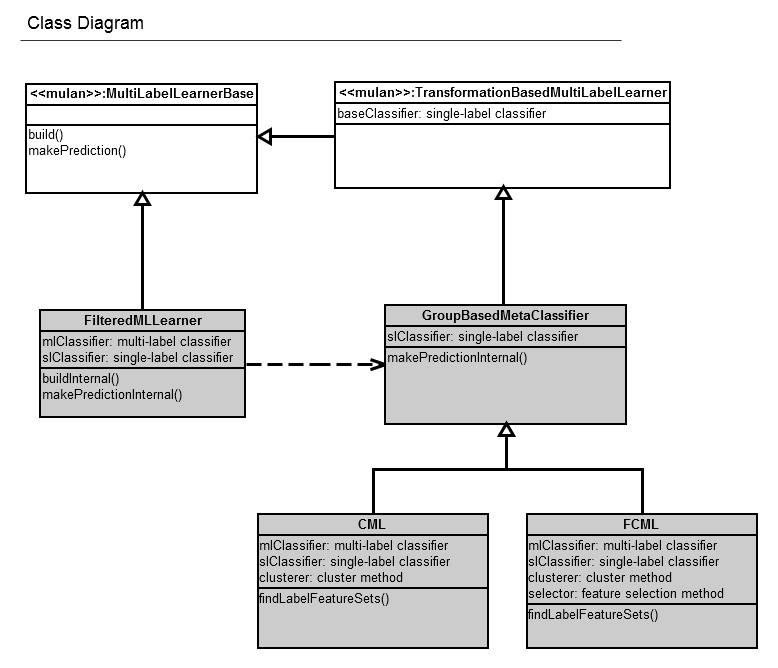
\includegraphics[width=\textwidth]{classdiagramm.png} 
			\caption{Class diagram showing the implementation structure of this work: self implemented classes are grey, white boxes represent \mbox{MULAN} classes. Most important input and output methods are shown. Drawn through lines indicate an "extends"-relationship, dashed lines an "used-by"-relationship.\newline Main class is the \textit{GroupBasedMetaClassifier} as it holds the subsets of the data "groups" and the multi-label classifier as well the single-label classifier. For every group a \textit{FilteredMLLearner} is used to extract the group subset from the dataset. For identifying groups either \textit{CML} or \textit{FCML} is used.}
		    \label{img:classDiag}
		\end{figure}

	\section{Multi-Label Datasets}
	\label{sec:datasets}

		A dataset can be described as $ N \times L \times M$ where $N$ is the number of instances, $ L $ the number of labels and $ M $ the number of features. \textit{Bibtex} and \textit{Delicious} are very large datasets in both label set cardinality and number of instances. This leads to very long computational times for clustering and feature selection. Therefore, those datasets where only tested with a small number of settings.

		In table \ref{tab:datasets} all datasets used in this work are presented. Additionally to their dimensions and type, the label cardinality ($LCard$) and  density ($LDens$) \cite{Tsoumakas07} of the dataset are shown. Both values measure the distribution of labels associated with an instance.

		\begin{equation}
			\label{LCard}
			LCard(D)=\frac{\sum_{i=1}^N|y_i|}N
		\end{equation}
		
		\textit{Label Cardinality} ($LCard$) (see equation \ref{LCard}) is the average number of labels associated with each instance.
		
		\begin{equation}
			\label{LDens}
			LDens(D)=\frac 1N LCard(\mathcal D)
		\end{equation}
		
		\textit{Label Density} ($LDens$) (see equation \ref{LDens}) is the average fraction of the label space associated with an instance. 
		
		\begin{table}
			\begin{center}
				\begin{tabular}{ c || c | c | c | c | c | c }
					& $N$ & $L$ & $M$ & $LCard$ & $LDens$ & type \\ \hline\hline
					Yeast & 2417 & 14 & $103n$ & 4.24 & 0.30 & biol.\\ \hline
					Medical & 978 & 45 & $1449b$ & 1.25 & 0.03 & text \\ \hline
					Enron & 1702 & 53 & $1001b$ & 3.38 & 0.06 & text \\ \hline\hline
					Bibtex & 7395 & 159 & $1836b$ & 2.40 & 0.02 & text \\ \hline
					Delicious & 16105 & 983 & $500b$ & 19.02 & 0.02 & text \\
				\end{tabular}
				\caption{Multi-label datasets used in this work. $N$ is the number of instances, $L$ the number of Labels. $M$ is the number of Features. $n$ indicates numeric features, $b$ binary features}
				\label{tab:datasets}
			\end{center}
		\end{table}

		In the following, datasets are described in more detail.

		\textit{Yeast} \cite{DBLP:conf/nips/ElisseeffW01} is a small biological dataset mapping genes to subsets of 14 different biological functions.

		\textit{Medical} \cite{Pestian07w.:a} was created for the Computational Medicine Centers 2007 Medical Natural Language Processing Challenge\footnote{\url{http://www.computationalmedicine.org/challenge/}}. The instances are compiled out of brief medical reports containing symptom and their prognosis labeled with insurance codes.

		\textit{Enron} \cite{read:2008} is a subset of the the Enron e-mail corpus\footnote{\url{http://bailando.sims.berkeley.edu/enron/}} hierarchically labeled with categories by the UC Berkley Enron Email Analysis Project\footnote{\url{http://bailando.sims.berkeley.edu/enron_email.html}}.

		\textit{Delicios} \cite{Tsoumakas08} is a collection from the \textit{del.ico.us} social bookmarking site\footnote{\url{http://del.ico.us}}. Every posted site on this bookmarking site is annotated with different tags. Tsoumakas \textit{et al.} filtered the set of overall 22139 tags to 983 frequent tags. In a second steps a boolean bag-of-word model for each bookmarked site was created and associated with the tags. In contrast to most other multi-label datasets in this context, labels were known prior to the feature space (bag-of-word model).

	\section{Evaluation Measures}
	\label{sec:evalmeasures}
	
		Evaluation in multi-label classification differs from single-label evaluation: The latter is the simple decision if a prediction of a single class is right or wrong. The result can be easily stored in a confusion matrix. Measures like specificity, the fraction of true negatives in all negatives and sensitivity, the fraction of true positives in all positives had been known for a long time in this area.

		For multi-label problems, a strict right/wrong evaluation criteria would be very harsh as predictions of label sets would be counted as wrong if any false positive or false negative would occure, disregarding other correct predictions. Thus additional measures for multi-label prediction were introduced.

		Two general fashions of multi-label evaluation measures exist: example-based measures where each predicted example is evaluated separately and label-based measures which are evaluating the binary relevance of each label individually \cite{citeulike:8938538}.

		A transfer of the classic single label \textit{accuracy} into multi-label application inducts a measure $SubsetAccuracy(D)$ (equation \ref{eqn:subsetaccuracy}) \cite{Ghamrawi05collectivemultilabel} as an example-based measure. $HammingLoss(D)$ (equation \ref{eqn:hammingloss}) \cite{Schapire00boostexter:a} would be the label-based equivalent.
	
		\paragraph{Example-based Evaluation Measures}
			\label{para:examplemeasures}
			
			In this paragraph $D$ is a dataset of testing, i.e. unseen examples. $N$ denotes the number of examples, $L$ the number of labels. $\hat{Y_i}$ is the predicted label set, $Y_i$ is the known true label assignment. 

			\begin{equation}
				\label{eqn:subsetaccuracy}
				SubsetAccuracy(D) = \frac{1}{N} \sum_{i=1}^{N} 1_{\hat{Y_i}=Y_i}
			\end{equation}
			
			\textit{SubsetAccuarcy} is the fraction of correct predicted label sets.

			\begin{equation}
				\label{eqn:hammingloss}
				HammingLoss(D) = \frac{1}{NL} \sum_{i=1}^{N} |\hat{Y_i}\Delta Y_i|\footnote{$A\Delta B$ is the symmetrical difference between $A$ and $B$ (logical XOR)\\ $0\Delta 0 = 1, 1\Delta0 = 1, 0\Delta 1 = 1, 1\Delta 1 = 0$}
			\end{equation}

			\textit{HammingLoss} is the failure (loss) in the predicted label sets averaged over instances $N$ and labels $L$.

		\paragraph*{} 
		\label{para:otherexample}		
			
			Other single label measures were adapted for multi-label use \cite{Godbole04discriminativemethods}:

			\begin{equation}
				\label{eqn:precision}
				Precision(D) = \frac{1}{N} \sum_{i=1}^{N} \frac{|\hat{Y_i}\vee Y_i|}{|\hat{Y_i}|}
			\end{equation}
				
			\textit{Precision} is the fraction of predicted labels which are relevant.

			\begin{equation}
				\label{eqn:recall}
				Recall(D) = \frac{1}{N} \sum_{i=1}^{N} \frac{|\hat{Y_i}\vee Y_i|}{|Y_i|}
			\end{equation}

			\textit{Recall} is the fraction of labels which are relevant and are also predicted.

			\begin{equation}
				\label{eqn:fmeasure}
				F-Measure(D) = \frac{1}{N} \sum_{i=1}^{N} \frac{2|\hat{Y_i}\vee Y_i|}{|\hat{Y_i}|+|Y_i|}
			\end{equation}

			\textit{F-Measure} is the weighted average of precision and recall. 

			\begin{equation}
				\label{eqn:accuracy}
					Accuracy(D) = \frac{1}{N} \sum_{i=1}^{N} \frac{|\hat{Y_i}\wedge Y_i|}{|\hat{Y_i}\vee Y_i|}
			\end{equation}

				\textit{Accuracy} is the fraction of union and intersection of predicted and real label sets for each instance and averaged over the number of examples. 

			\paragraph*{Label-based Evaluation Measures}
				\label{para:labelmeasures}

				For label-based evaluation measures, any binary evaluation measure can be used. The only difference is the averaging process, as multi-label applications offer two ways of averaging: \textit{macro-averaging} and \textit{micro-averaging} \cite{Yang99anevaluation}. A binary evaluation $ M(tp,tn,fp,fn)$ uses the number of true positives ($tp$), true negatives ($tn$), false positives and false negatives ($fp$ and $fn$) as input. Those numbers can be averaged as follows:
				\begin{equation}
					\label{eqn:mmacro}
					M_{macro}=\frac{1}{L}\sum_{i=1}^L M({tp}_i,{tn}_i,{fp}_i,{fn}_i)
				\end{equation}

				\begin{equation}
					\label{eqn:mmacro}
					M_{micro}=\frac{1}{L} M(\sum_{i=1}^L {tp}_i,\sum_{i=1}^L {tn}_i,\sum_{i=1}^L {fp}_i,\sum_{i=1}^L {fn}_i)
				\end{equation}

	\section{Evaluation of Clustering- and Feature Selection Methods}
		\label{sec:evaluation}

		In order to achieve best results for CML (section \ref{sec:CML}) or FCML (section \ref{sec:FCML}), an ideal clustering and feature selection method has to be selected. Several algorithms and combinations were evaluated, each by a 5-fold cross-validation on various datasets. The numerous parameters for both, clustering and feature selection, lead to a very high number of evaluations with partially very long run times. Over $30.000$ different settings were computed at the BIMComputeCluster\footnote{\url{http://www.bioinformatik-muenchen.de/studium/students/bim-compute-cluster}} and the Linux-Cluster at the Leibniz-Rechenzentrum\footnote{\url{http://www.lrz.de/services/compute/linux-cluster/}}. 

		\subsection{Clustering}
			\label{subsec:eval_clustering}

			Clustering is crucial for the performance of FCML and CML. This section shows different evaluation settings for clustering and its results.

			For distance based cluster methods such as hierarchical clustering and simple k-means (section \ref{subsubsec:kmeans}), a distance metric has to be chosen. Those methods also need the number of clusters $nc$ to be specified. Furthermore, hierarchical clustering needs a linkage criterion to be given. This results in a very high number of evaluation settings. To average cluster performance, different feature selection methods and number of clusters, as well varying datasets are used.

				\paragraph{CML} In figure \ref{fig:cml_clus} clustering results for CML are shown. EM is outperformed by distance-based cluster methods. The EM algorithm is based on the Maximum-Likelihood-Principle, though for this application distance measures have advantages for the use as similarity measure for attributes. Regarding the distance measures, the \textit{Chebyshev} distance shows disadvantages, while \textit{Euclidean} and \textit{Manhattan} distances seem to perform equally well. The latter ones are more sensitive to cumulative differences in many values, but less sensitive to single large differences. \textit{Chebyshev} regards only the maximum distance between two instances, hence it is very receptive to outliers. Considering hierarchical cluster methods, \textit{single, complete} and \textit{average} linkage show equal performance. \textit{Mean} has an average accuracy about 15\% lower. Note that \textit{Chebyshev} does not have disadvantages in \textit{mean} linkage scenarios. \textit{Mean}-linkage is also very sensitive to outliers, as the distance to every other instance is summed up.

				\paragraph{FCML} More detailed results for FCML are shown in figure \ref{fig:fcml_clus}. In comparison to CML, EM does not show a significant disadvantage versus distance based cluster methods. FCML does use scores computed from a feature selection method. Those scores are expectable to be distributed along some probability distribution. In the \textit{medical} dataset EM shows improvements against hierarchical and k-means clustering. Despite this exception, no overall "best-performing" cluster method could be determined although hierarchical clustering shows enhancements in some cases. A closer look at the hierarchical clustering is done in figure \ref{fig:fcml_clus_meth} and \ref{fig:fcml_clus_dist}. One can see again, there are no bold differences in neither, distance measure nor cluster method. 

					To overcome the problem of a missing standard setting working well for every scenario, a ranking for each scenario (dataset \& multi-label learner) has been created. Settings were ordered along their example-based accuracy. Tables \ref{tab:cal500}, \ref{tab:enron}, \ref{tab:medical} and \ref{tab:yeast} show the top 3 settings for the datasets \textit{cal500}, \textit{enron}, \textit{medical} and \textit{yeast}. Ranking differ between datasets but \textit{HierarchicalClusterer} using single-linkage is among all top 3 results, thus further evaluation will use this setting.

				\begin{table}\tiny
					\centering
					\subtable[ranking in dataset \textit{CAL500}\label{tab:cal500}]{
				    	\begin{tabular}{rrrrrr}
					    	\toprule
								rank  &  multi-label learner & feature-selection method & cluster algorithm & cluster method & distance measure \\
						    \midrule
						    \#1   &  ClassifierChain & InfoGainAttributeEval & SimpleKMeans & & ManhattanDistance \\
						    \#2   &  ClassifierChain & InfoGainAttributeEval & HierarchicalClusterer & SINGLE & ChebyshevDistance \\
						    \#3   &  ClassifierChain & InfoGainAttributeEval & HierarchicalClusterer & SINGLE & EuclideanDistance \\
						    \bottomrule
					    \end{tabular}%
				    }
				    \subtable[ranking in dataset \textit{enron}\label{tab:enron}]{
						\begin{tabular}{rrrrrr}
						    \toprule
								rank  &  multi-label learner & feature-selection method & cluster algorithm & cluster \\  method & distance measure \\
						    \midrule
						    \#1   &  ClassifierChain & InfoGainAttributeEval & HierarchicalClusterer & SINGLE & SpearmanCoefficient \\
						    \#2   &  ClassifierChain & InfoGainAttributeEval & HierarchicalClusterer & MEAN  & SpearmanCoefficient \\
						    \#3   &  ClassifierChain & InfoGainAttributeEval & HierarchicalClusterer & COMPLETE & SpearmanCoefficient \\
						    \bottomrule
					    \end{tabular}
				    }
					\subtable[ranking in dataset \textit{medical}\label{tab:medical}]{
						\begin{tabular}{rrrrrr}
						    \toprule
							rank  &  multi-label learner & feature-selection method & cluster algorithm & cluster method & distance measure \\
							\midrule
						    \#1   &  ClassifierChain & InfoGainAttributeEval & SimpleKMeans &       & EuclideanDistance \\
						    \#2   &  ClassifierChain & InfoGainAttributeEval & SimpleKMeans &       & ManhattanDistance \\
						    \#3   &  ClassifierChain & InfoGainAttributeEval & HierarchicalClusterer & SINGLE & ManhattanDistance \\
						    \bottomrule
					    \end{tabular}
				    }
				    \subtable[ranking in dataset \textit{yeast}\label{tab:yeast}]{
						\begin{tabular}{rrrrrr}
						    \toprule
							 rank  &  multi-label learner & feature-selection method & cluster algorithm & cluster method & distance measure \\
							\midrule
						    \#1   &  ClassifierChain & InfoGainAttributeEval & SimpleKMeans &       & EuclideanDistance \\
						    \#2   &  ClassifierChain & InfoGainAttributeEval & SimpleKMeans &       & ManhattanDistance \\
						    \#3   &  ClassifierChain & InfoGainAttributeEval & HierarchicalClusterer & SINGLE & ManhattanDistance \\
						    \bottomrule
					    \end{tabular}
					}
					\caption{Ranking of scenarios within different datasets using ClassifierChain as multi-label learner. Only the Top 3 results are shown. Different feature selection methods as well different cluster algorithm were used. The results are ordered along their example-based accuracy.}
					\label{tab:ranking}
				\end{table}

				\begin{figure}
					\centering
					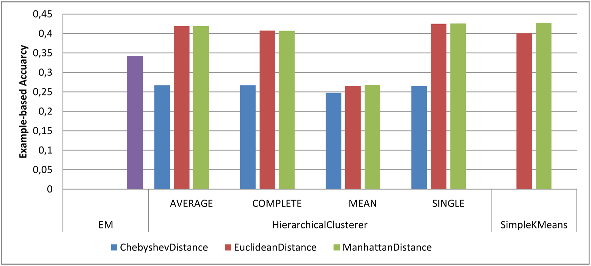
\includegraphics{figures/cml_cluster.pdf}
					\caption{Average Example-based accuracy for different cluster algorithm on CML over different datasets}
					\label{fig:cml_clus}
				\end{figure}

				\begin{figure}
					\centering			
					\subfigure[\scriptsize{Example-based Accuracy}]{
						\label{fig:fcml_clus_acc}
						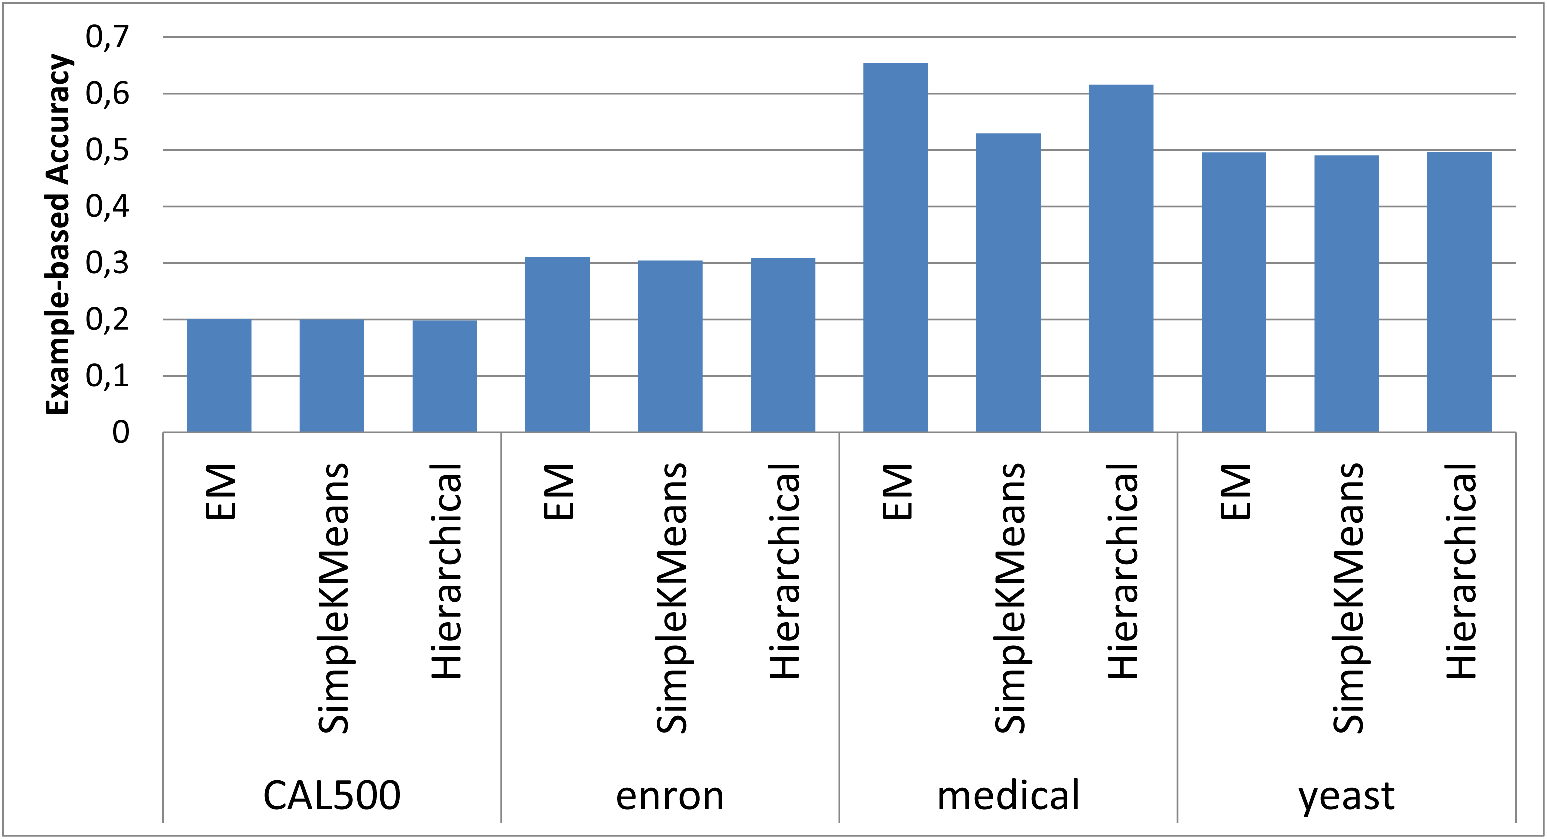
\includegraphics[width=.44\textwidth]{figures/fcml_cluster_acc.pdf}
					}
					\subfigure[\scriptsize{Micro-averaged F-Measure}]{
						\label{fig:fcml_clus_fmeasure}
						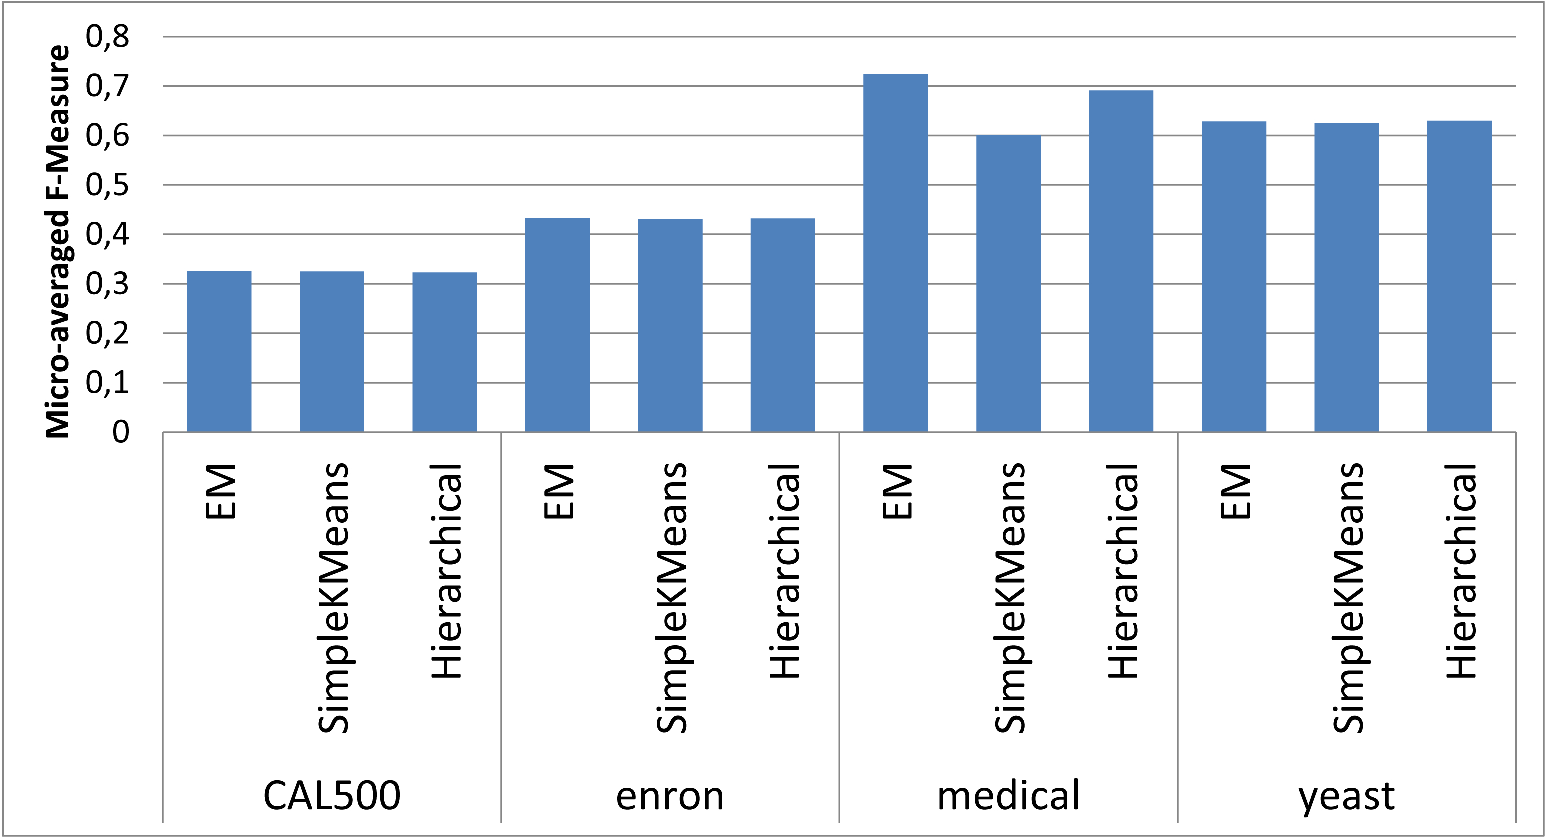
\includegraphics[width=.44\textwidth]	{figures/fcml_cluster_fmeasure.pdf}
					}
					\subfigure[\scriptsize{Hamming Loss}]{
						\label{fig:fcml_clus_hamming}
						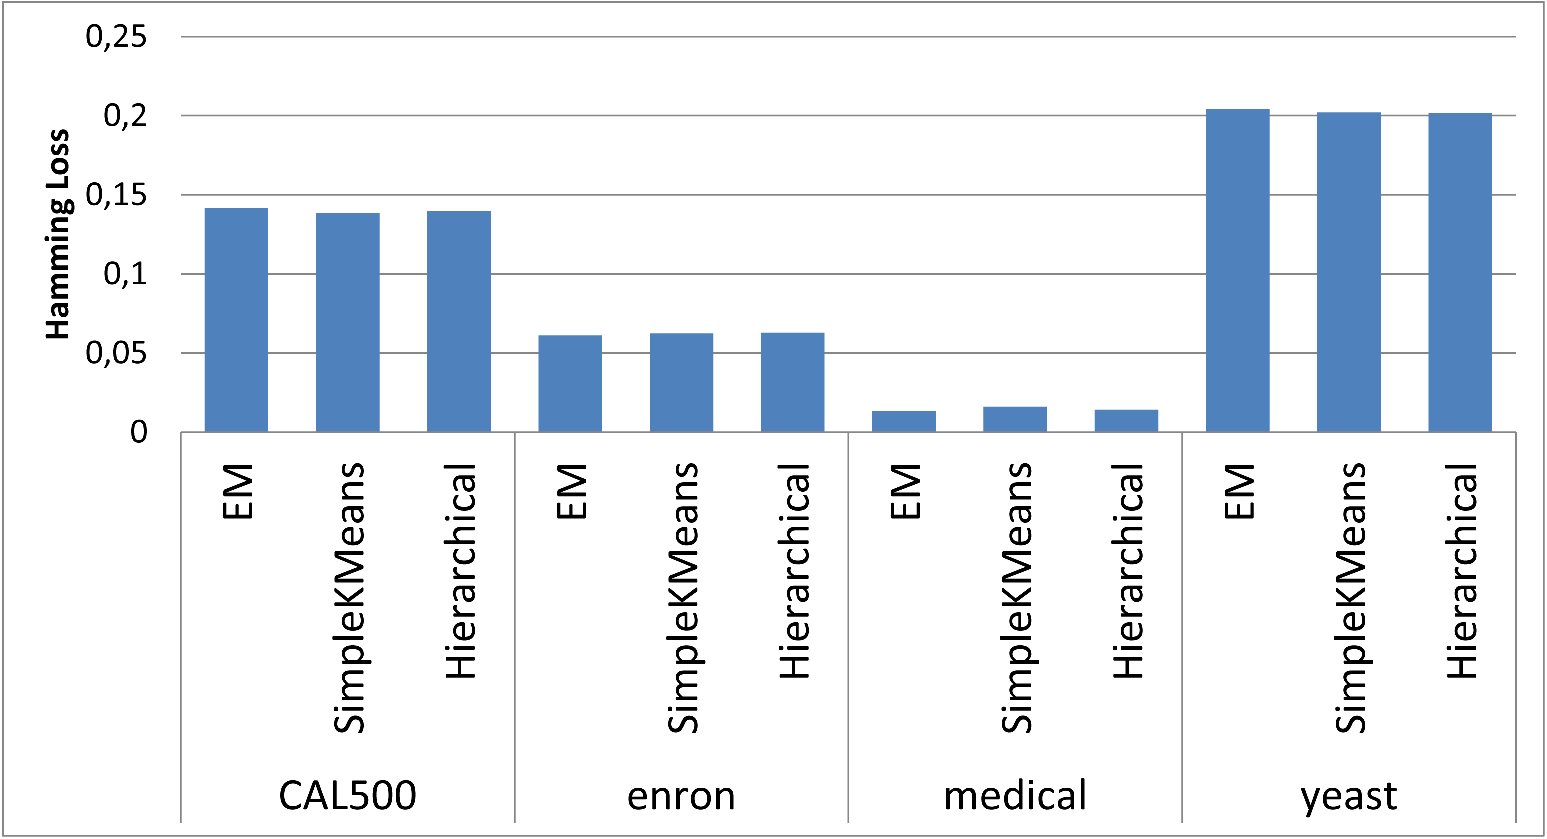
\includegraphics[width=.44\textwidth]{figures/fcml_cluster_hamming.pdf}
					}
					\caption{Evaluation of clustering algorithms in FCML. Different datasets were used. The measures are averaged over different settings, like $nc$, linkage criteria and distance measure}
					\label{fig:fcml_clus}
				\end{figure}

				\begin{figure}
					\centering			
					\subfigure[\scriptsize{Example-based Accuracy}]{
						\label{fig:fcml_clus_meth_acc}
						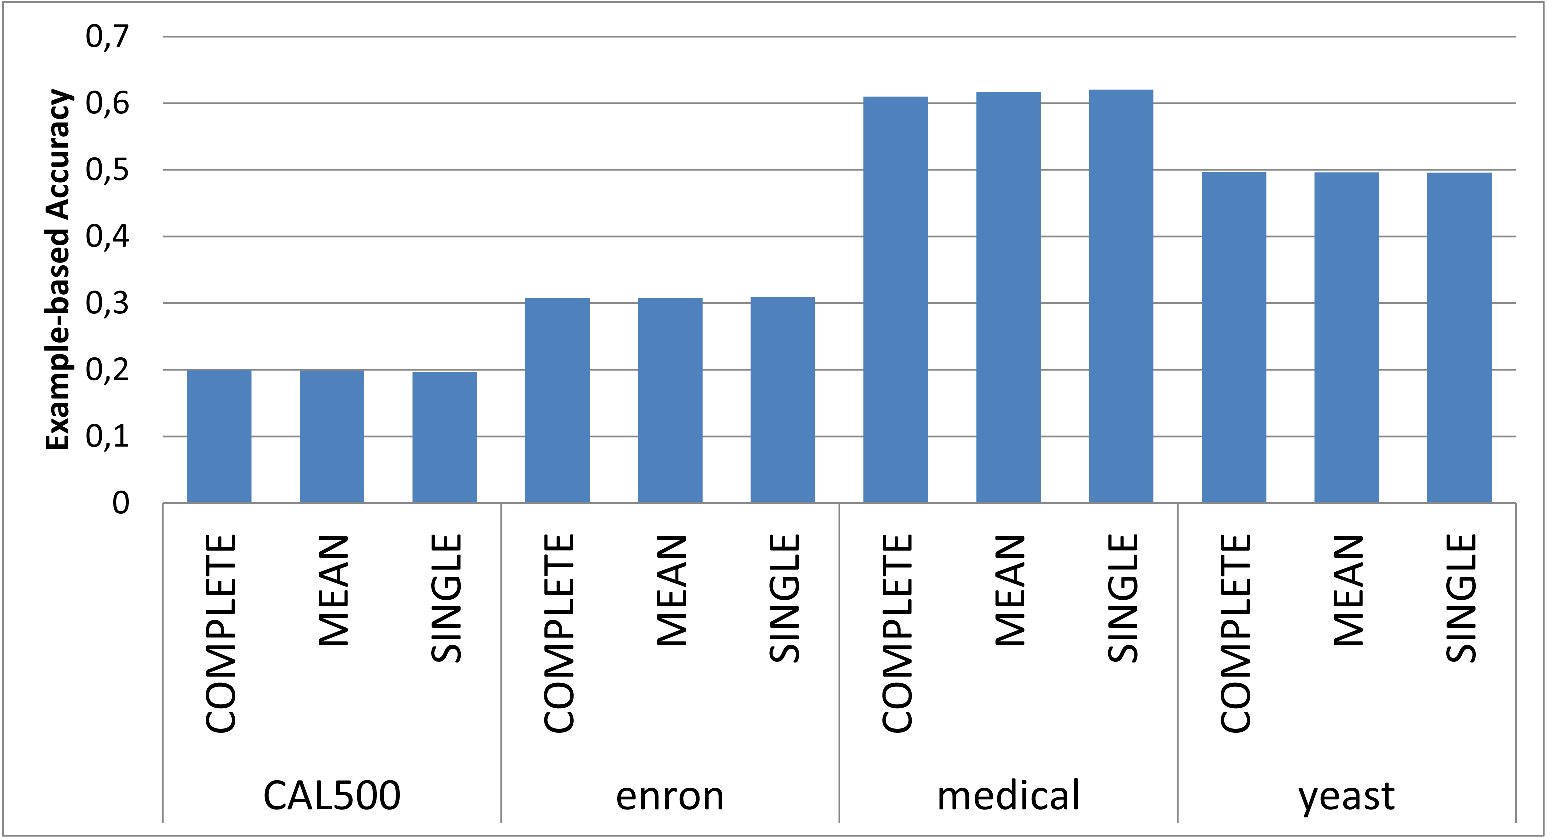
\includegraphics[width=.44\textwidth]{figures/fcml_clus_meth_acc.pdf}
					}
					\subfigure[\scriptsize{Micro-averaged F-Measure}]{
						\label{fig:fcml_clus_meth_fmeasure}
						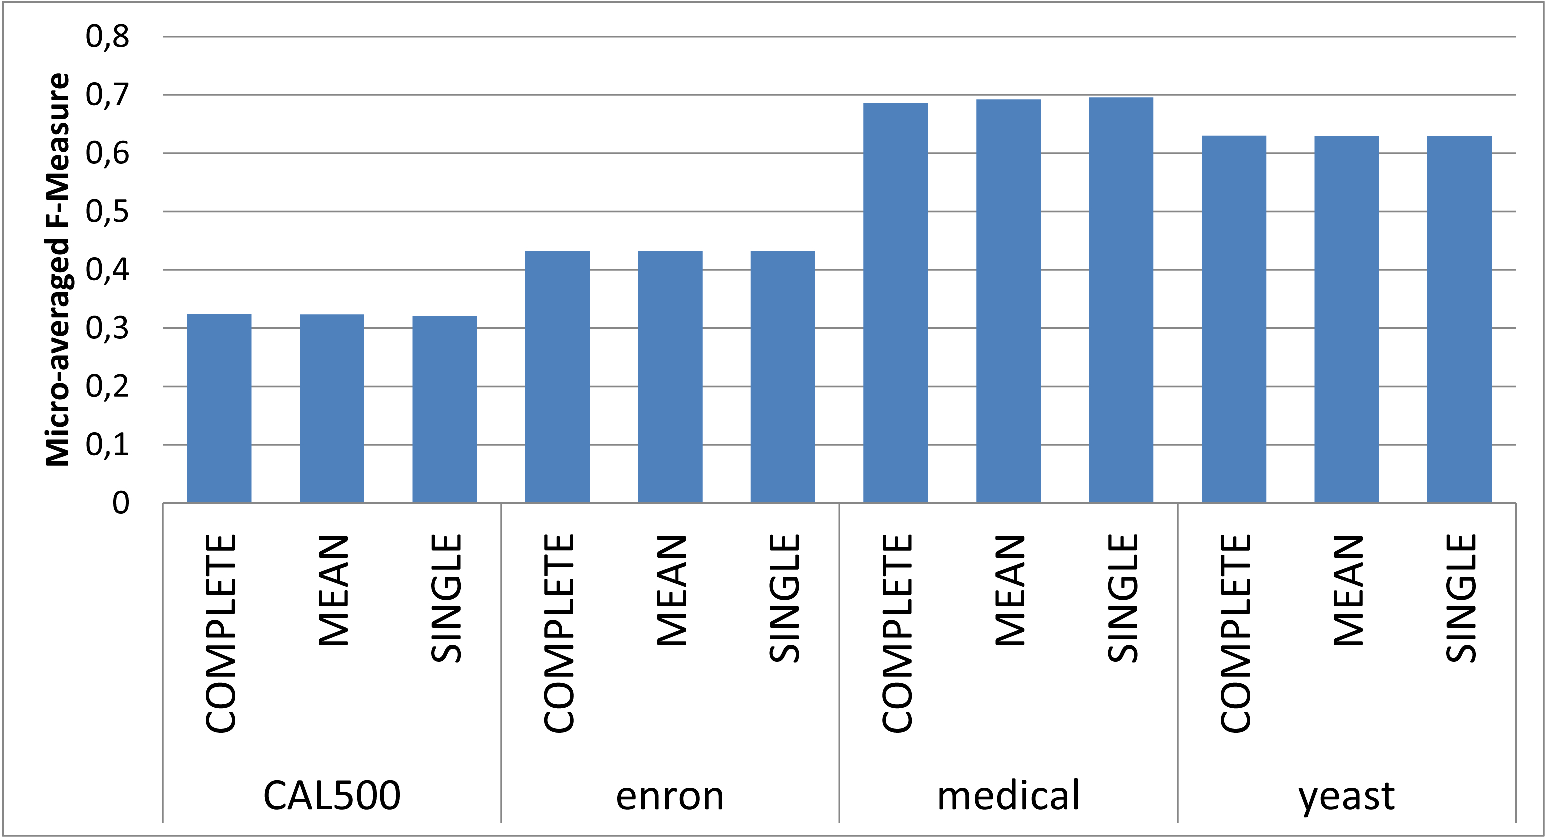
\includegraphics[width=.44\textwidth]	{figures/fcml_clus_meth_fmeasure.pdf}
					}
					\subfigure[\scriptsize{Hamming Loss}]{
						\label{fig:fcml_clus_meth_hamming}
						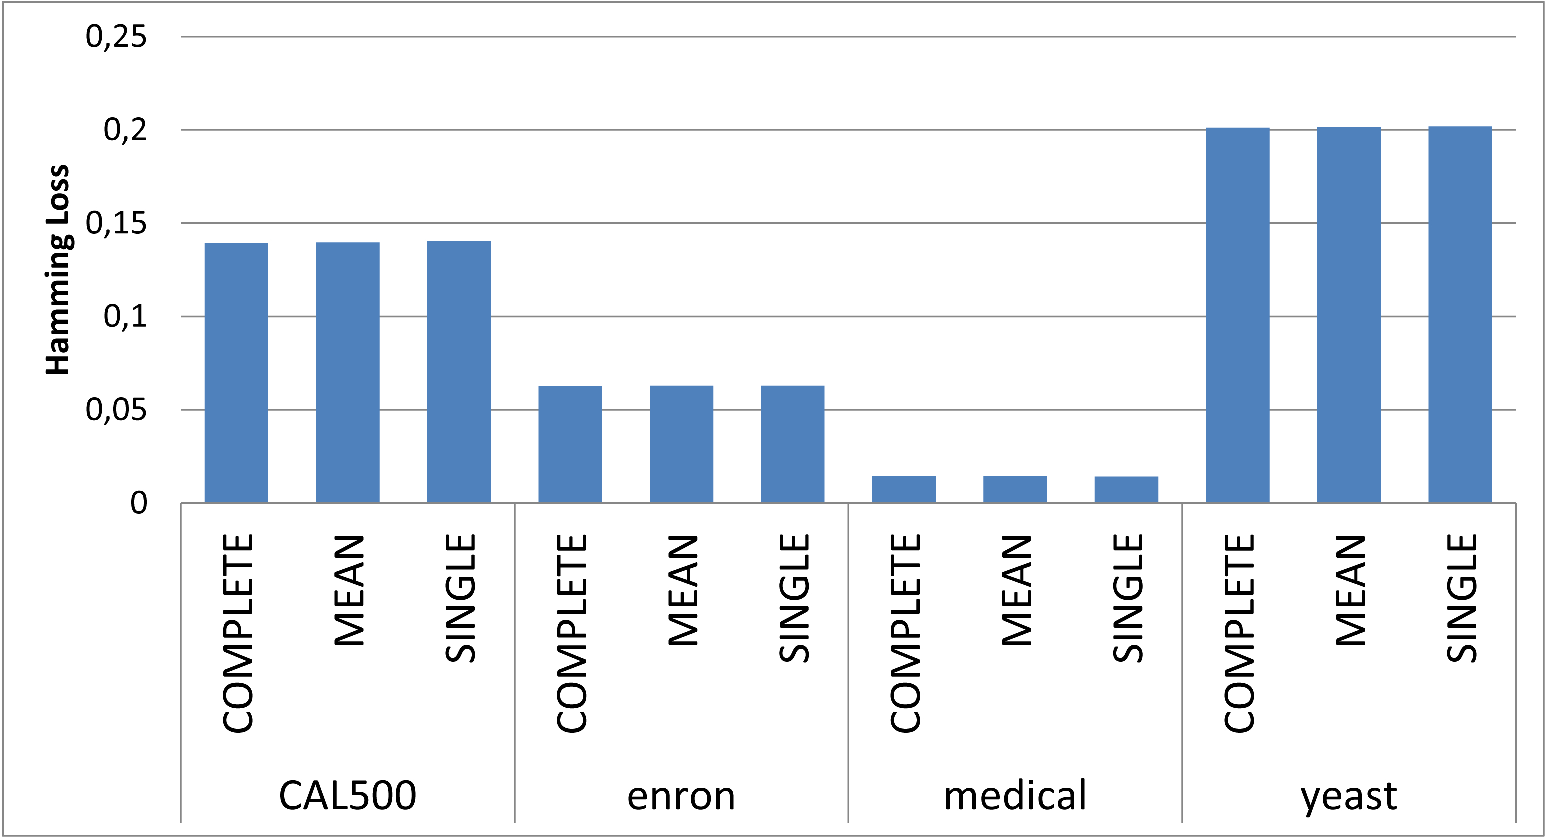
\includegraphics[width=.44\textwidth]{figures/fcml_clus_meth_hamming.pdf}
					}
					\caption{Evaluation of hierarchical clustering methods on different datasets. The measures are averaged over different distance measures}
					\label{fig:fcml_clus_meth}
				\end{figure}
					
				\begin{figure}
					\centering			
					\subfigure[\scriptsize{Example-based Accuracy}]{
						\label{fig:fcml_clus_dist_acc}
						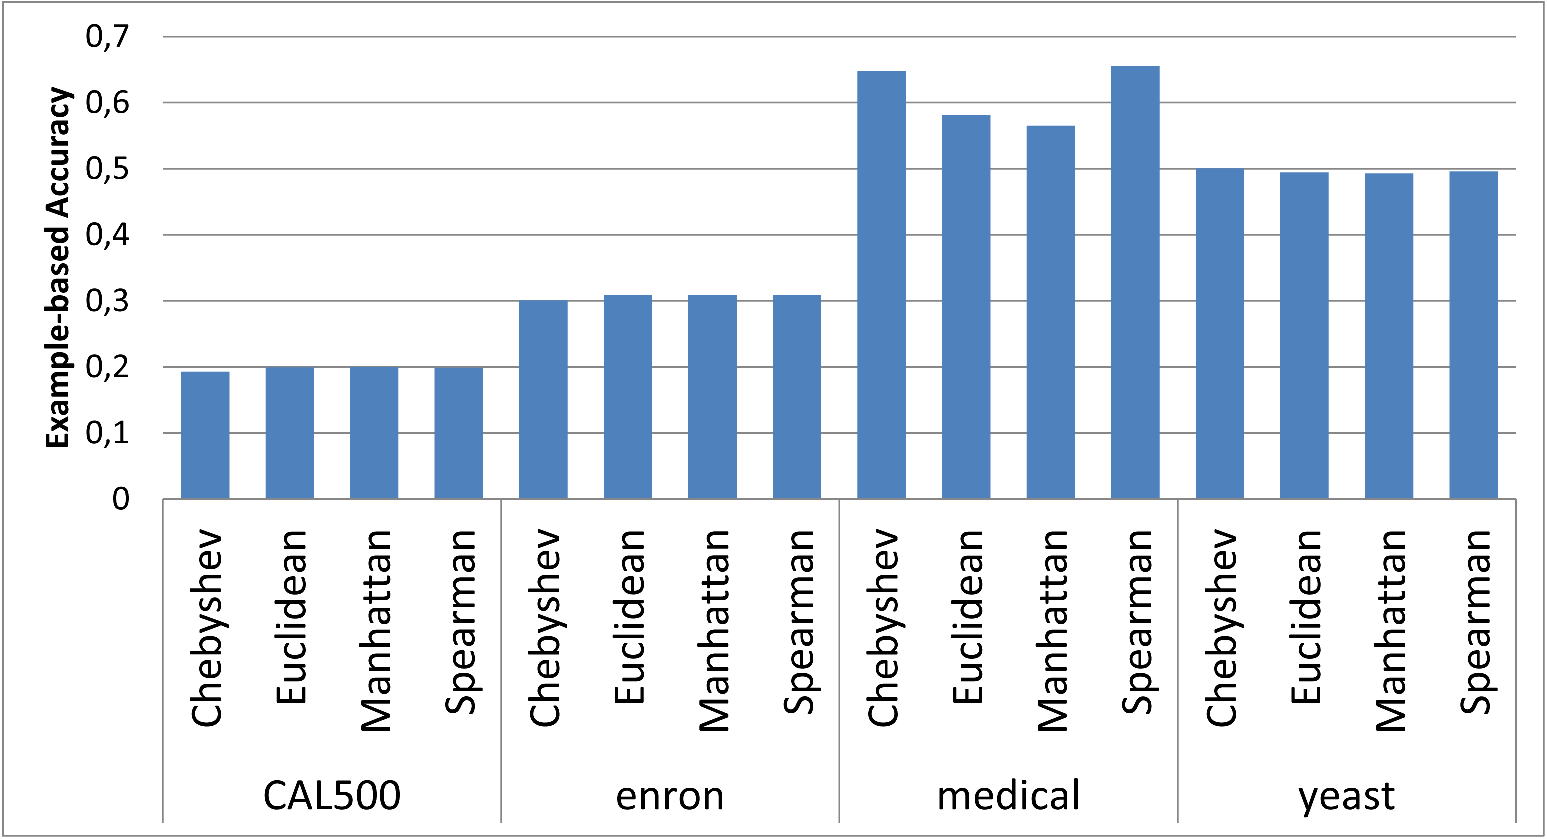
\includegraphics[width=.44\textwidth]{figures/fcml_clus_dist_acc.pdf}
					}
					\subfigure[\scriptsize{Micro-averaged F-Measure}]{
						\label{fig:fcml_clus_dist_fmeasure}
						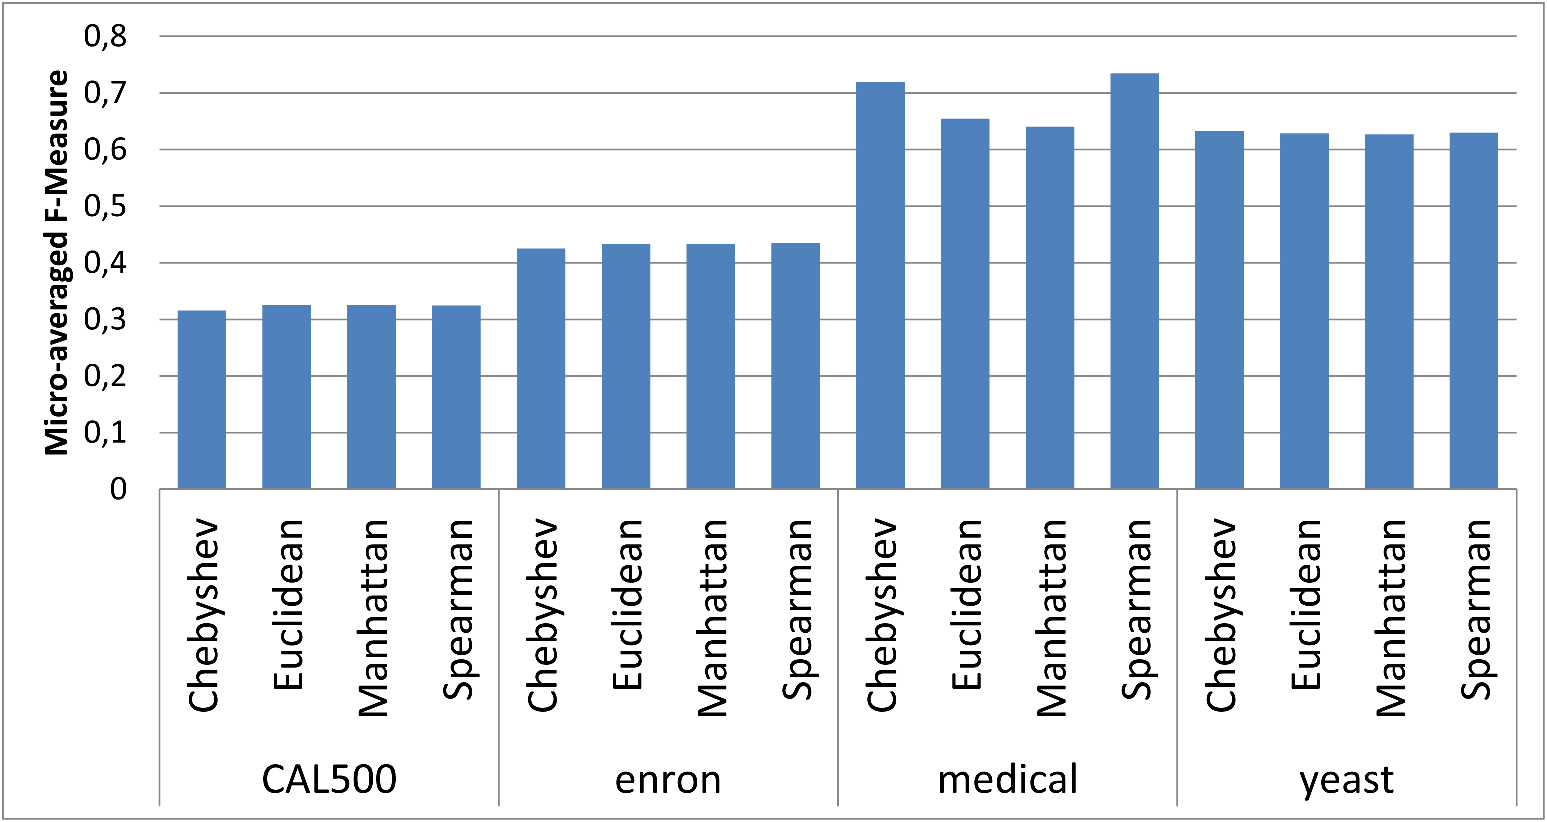
\includegraphics[width=.44\textwidth]	{figures/fcml_clus_dist_fmeasure.pdf}
					}
					\subfigure[\scriptsize{Hamming Loss}]{
						\label{fig:fcml_clus_dist_hamming}
						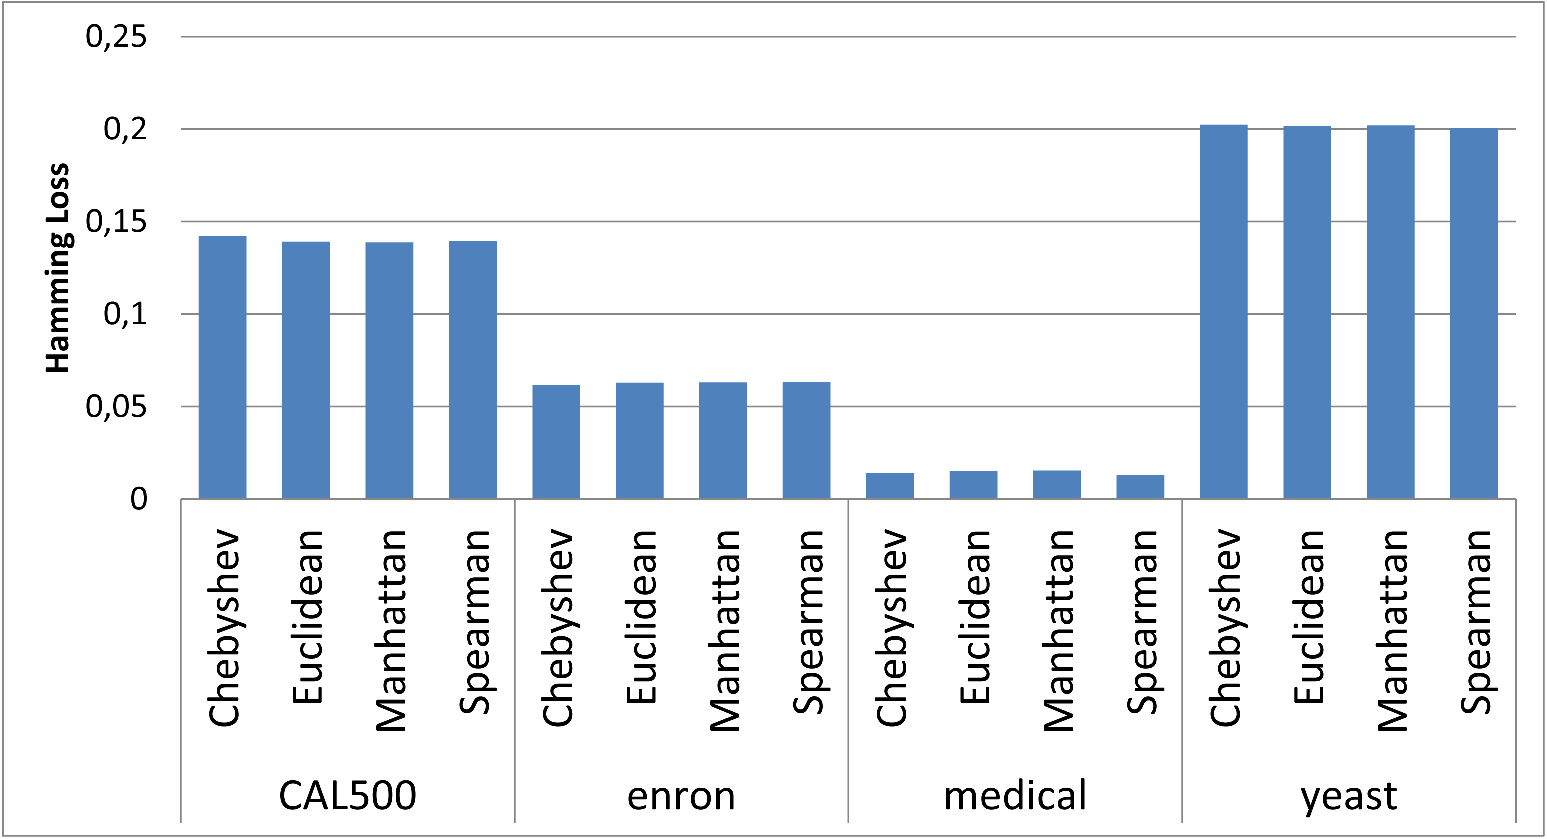
\includegraphics[width=.44\textwidth]{figures/fcml_clus_dist_hamming.pdf}
					}
					\caption{Evaluation of distance measure using hierarchical clustering on different datasets. The measures are averaged over different distance measures}
					\label{fig:fcml_clus_dist}
				\end{figure}


				\paragraph*{Number of clusters} Finally the parameter "number of clusters" has to be identified. The number of clusters ($nc$) can range from at least 2 to $|L|$, which results in each label to be clustered in a single cluster. Therefore, $nc$ is highly related to the size of the dataset, where $|L|$ can be between 14 (\textit{yeast}) and 983 (\textit{delicious}).

				For finding rules for determining $nc$, several attempts to identify correlations between $nc$ and evaluation measures like \textit{accuracy} or dataset specific measures like \textit{label-density} were made. Figure \ref{fig:clu_cor} shows the result for the setting "ClassifierChain, Hierarchical Clustering, single-linkage, Euclidean Distance, InformationGain" on the dataset \textit{CAL500}.
					
				In table \ref{tab:cor} a correlation matrix between the measures \textit{Example-based Accuracy}, \textit{Micro-averaged F-Measure}, \textit{Hamming-Loss} and \textit{avgDensity} as well the average labels per cluster and the number of clusters itself is shown. \textit{avgDensity} is the density averaged over all groups. The correlation was computed from the values for each step for $nc$ from 2 to $|L|$.
					
				The matrix shows poor correlation, with an exception on "Hamming-Loss" to "avgDensity". As the best value in Hamming-Loss is 0, performance seems to decrease with higher average density. However, the reason for this relationship could not be covered in this work due to time limits.
 
				\begin{figure}
					\centering
					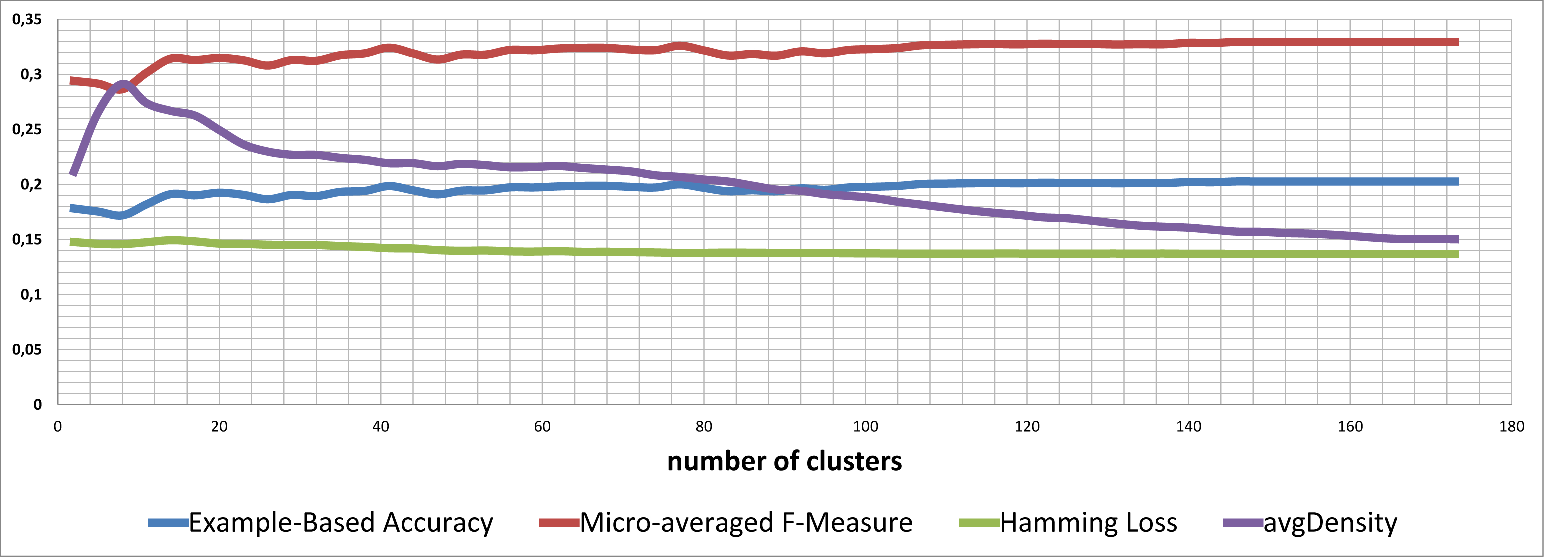
\includegraphics[width=.9\textwidth]{figures/cluster_corl.pdf}
					\caption{Example-based Accuracy, Micro-averaged F-Measure, Hamming Loss and average Density with growing number of clusters. The setting "ClassifierChain, Hierarchical Clustering, single-linkage, Euclidean Distance, InformationGain" \textit{CAL500} is used}
					\label{fig:clu_cor}
				\end{figure}

				\begin{table}\scriptsize
					\centering
					\begin{tabular}{r||r|r|r}
						& density & labels per cluster & number of clusters \\\hline\hline
						Accuracy & -0,2623 & -0,195886517 & -0,4528997 \\\hline
						F-Measure & -0,214 & -0,208032488 & -0,47366346 \\\hline
						HammingLoss & 0,78642 & 0,063797033 & 0,23463825 \\
					\end{tabular}
					\caption{Pearson-correlation matrix for the setting "ClassifierChain, Hierarchical Clustering, single-linkage, Euclidean Distance, InformationGain" \textit{CAL500} dataset with different $nc$}
					\label{tab:cor}
				\end{table}

		\subsection{Feature-Selection}

		FCML (see section \ref{sec:FCML}) uses feature selection methods to compute scores/ranks for every attribute. The configuration of the feature selection scenario is crucial to the learning and prediction process. 

		In order to isolate effects of ranking, in detail to ignore scores within the adding features to groups, any threshold is set to minimum. This leads to groups which only differ in the label subsets but always contain the entire features space. The evaluation of an optimal feature selection threshold is a separate task.
		
		To evaluate the feature selection process, a clustering algorithm is needed. To reduce the influence of good or bad clustering, various cluster algorithms and parameters were used. Finally, the performance of the FCML method is averaged.

		To reduce the number of evaluations, two scenarios where considered: Firstly, five feature selection methods were evaluated on one dataset, namely \textit{CAL500}. The results are shown in \ref{fig:fscal}. Although \textit{CfsSubsetEval} shows tiny improvements against other methods, no superior method could be determined.

		A second step evaluates three different feature selection methods on varying datasets: \textit{Relief}, \textit{CFS} and \textit{Information Gain}. Those three methods were chosen because they represent independent solution approaches. Results, as shown in figure \ref{fig:fs}, point out that CFS can outvalue both other methods only in the \textit{medical} dataset. Hence, Hamming-Loss shows no improvement.

		As no superior feature selection method could be found, further evaluation \textit{information gain} uses because of its simplicity. It computes mutual certainty for a pair of attributes satisfying the claim that groups consist of attributes which have strong mutual associations.
				
		\textit{Information gain} has also advantages in terms of computing time. Therefore, it allows more settings to be evaluated. Nevertheless, further evaluating and parameter optimization could lead to better results on certain datasets.

		\begin{figure}
			\centering
			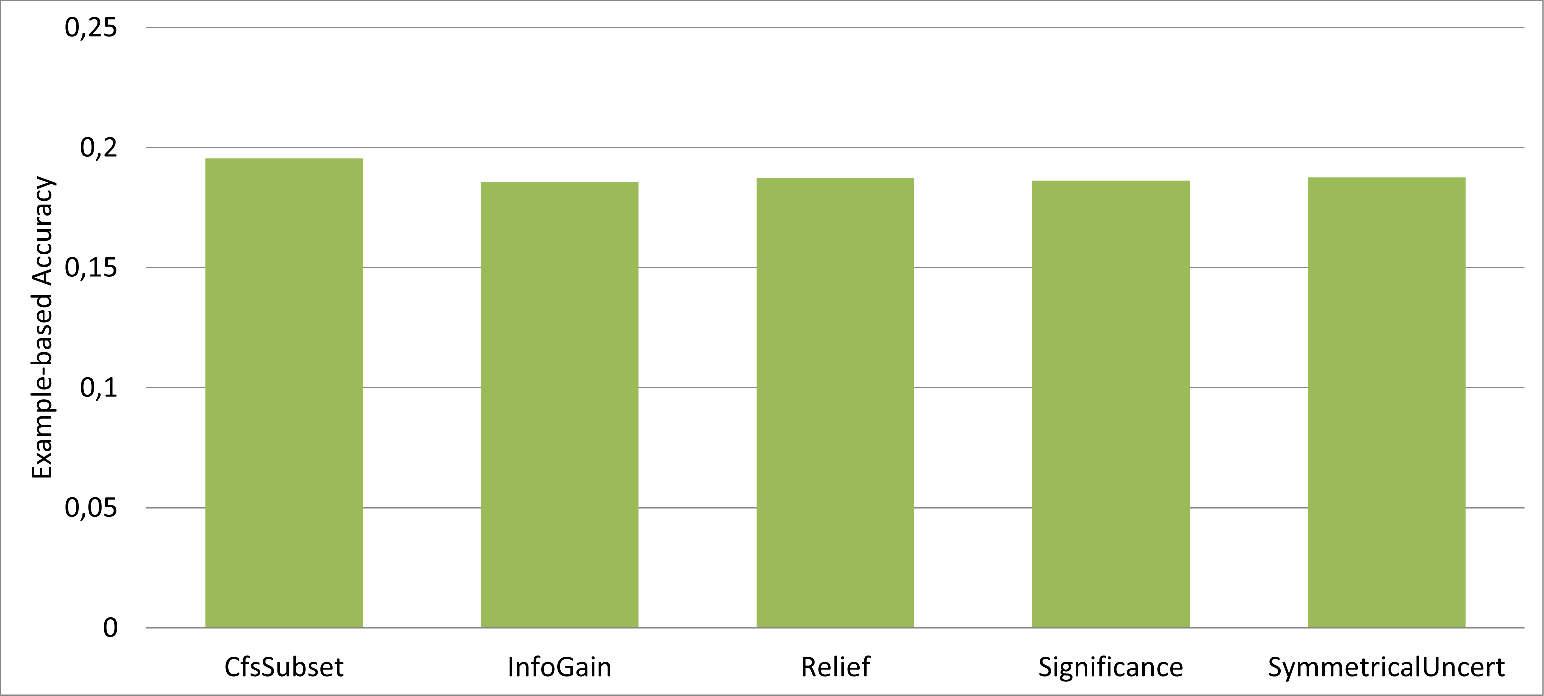
\includegraphics[width=.9\textwidth]{figures/five_fs.pdf}
			\caption{Feature-Selection Methods on the \textit{CAL500} dataset. Example-based Accuracy is averaged over different clustering settings}
			\label{fig:fscal}
		\end{figure}
				
		\begin{figure}
			\centering			
			\subfigure[\scriptsize{Example-based Accuracy}]{
				\label{fig:fcml_fs_acc}
				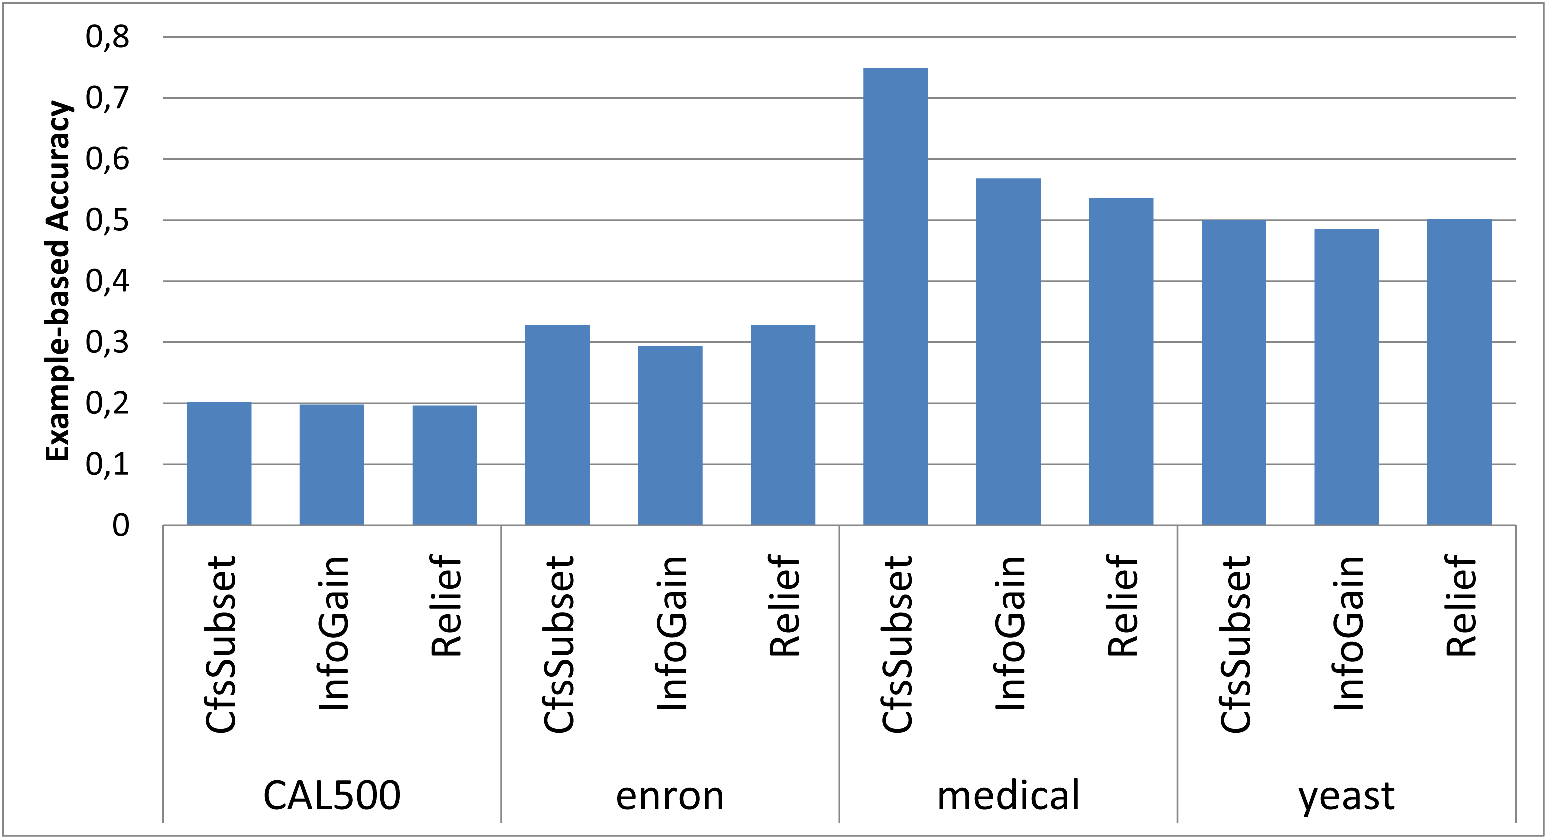
\includegraphics[width=.44\textwidth]{figures/fcml_fs_acc.pdf}
			}
			\subfigure[\scriptsize{Micro-averaged F-Measure}]{
				\label{fig:fcml_fs_fmeasure}
				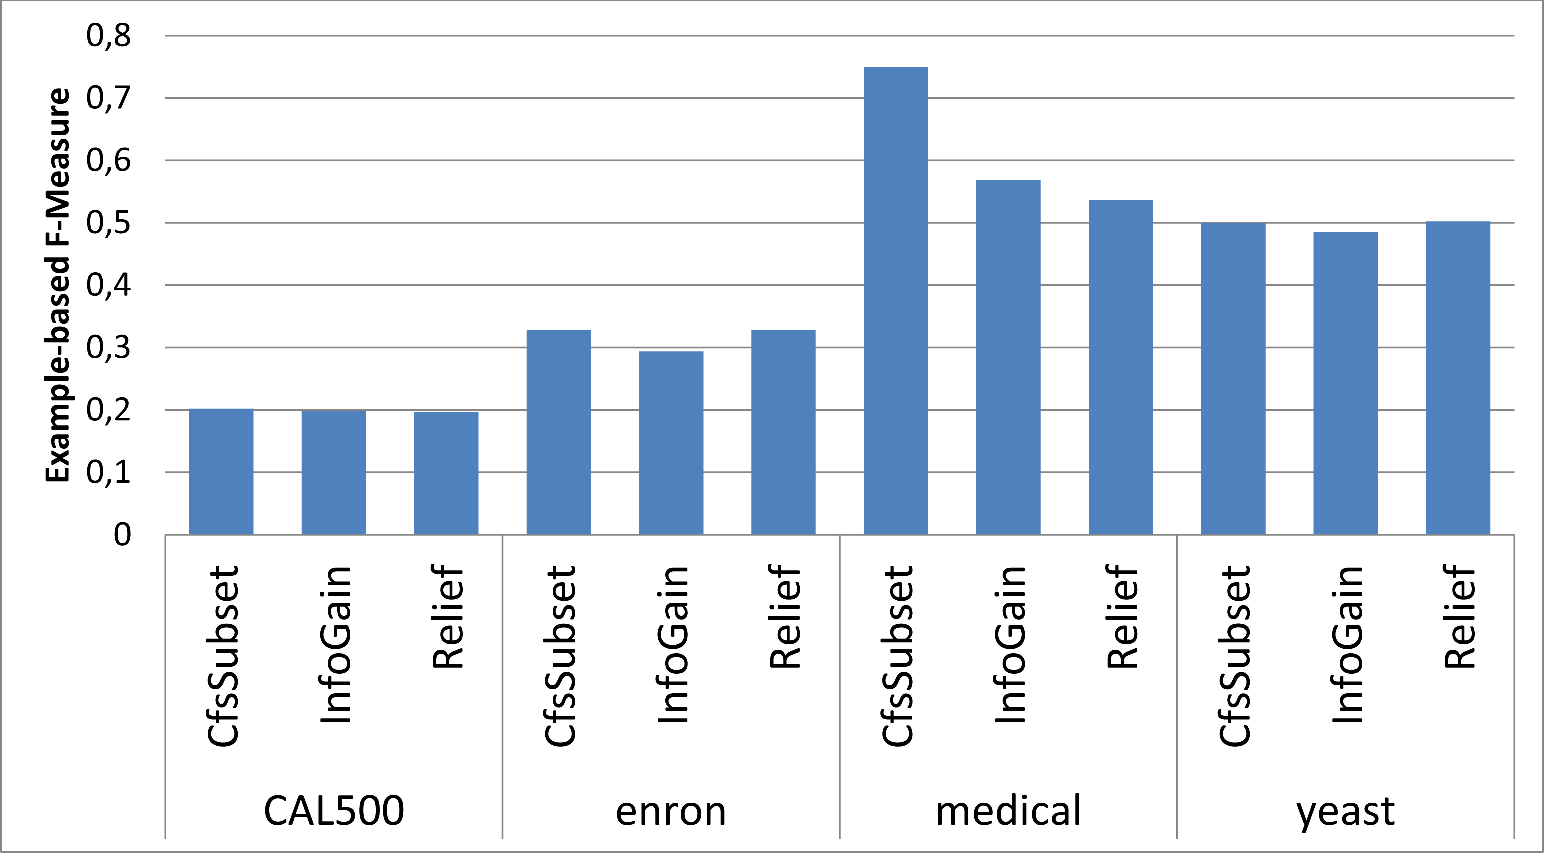
\includegraphics[width=.44\textwidth]	{figures/fcml_fs_fmeasure.pdf}
			}
			\subfigure[\scriptsize{Hamming Loss}]{
				\label{fig:fcml_fs_hamming}
				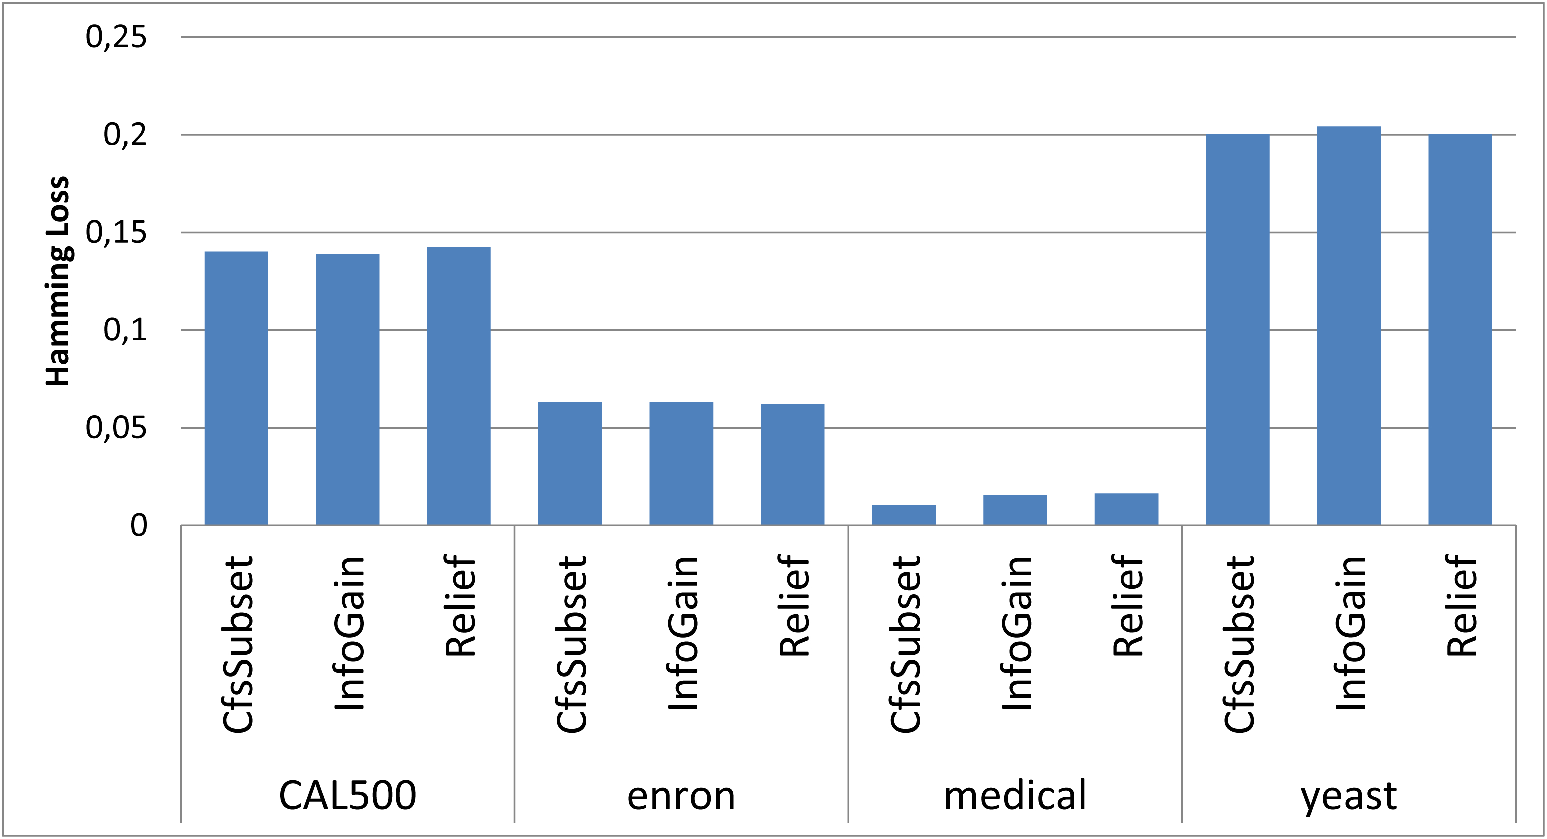
\includegraphics[width=.44\textwidth]{figures/fcml_fs_hamming.pdf}
			}
			\caption{\textit{Relief}, \textit{CFS} and \textit{Information Gain} feature selection on different datasets}
			\label{fig:fs}
		\end{figure}

	\subsection{Evaluation of methods}

		In the following, results from CML and FCML are presented. Note that CML was developed and tested prior to FCML, the latter one uses an extended set of datasets and evaluation techniques. Due to time limits it was not possible to repeat tests for CML with new datasets.

		\subsubsection{CML}

			\begin{figure}
				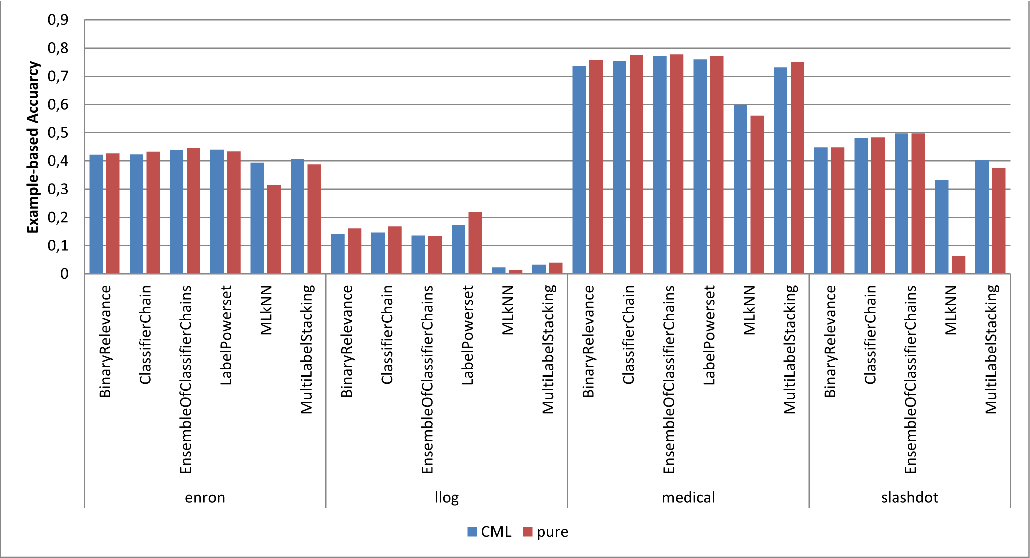
\includegraphics[width=\textwidth]{figures/cml_results.pdf}
				\caption{CML compared to pure multi-label learners using the example-based accuracy. For CML the best result is taken.}
				\label{fig:cml}
			\end{figure}

			In figure \ref{fig:fs} results of CML compared to pure multi-label learners are shown. If needed by the multi-label learner, a Support-Vector Machine (SMO) was used. As described before a hierarchical clustering with Euclidean distance measure and single-linkage was used. For the number of clusters, $nc$, different number of clusters, namely $2, 4, 6$, where chosen. For the results the best $nc$ was taken. All evaluation was done by a 5-fold cross-validation.

			Although nearly every scenario shows similar results for CML and the pure learner, performance of ML-kNN could be improved in every case.

			ML-kNN computes distances between instances and assigns query instance to the major label set of the k-nearest neighbors using a maximum-a-posteriori principle. Filtering the label space can enhance the MAP principle as the elements of the output label space are highly dependent and therefore MAP probabilities are likely to be high.

			In summery, CML can enhance the performance of multi-label learners in some cases, but on average CML shows the same performance as its pure multi-label scheme.

		\subsubsection{FCML}

			Results for FCML are shown in figure \ref{fig:fcml_res}. For every scenario (dataset + multi-label learner), all possible numbers of clusters $nc$ were evaluated and the best result is presented. To reduce the complexity of parameters, feature selection was used without threshold, e.g. groups always contain the entire feature space. HOMER, as described in section \ref{subsubsec:homer} was used for comparison. HOMER uses a parameter $k$ describing for the number of clusters at each hierarchical level. Every scenario, $k=2\hdots 8$ was evaluated and again the best result is presented. However, HOMER did not finish in every scenario due to memory limits (6GB) or problems in the implementation\footnote{IndexOutOfBounds-Exception during JAVA runtime}. In addition, for every scenario a pure multi-label learner has been trained.

			\begin{figure}
				\centering
				\subfigure[Example-based Accuracy]{
					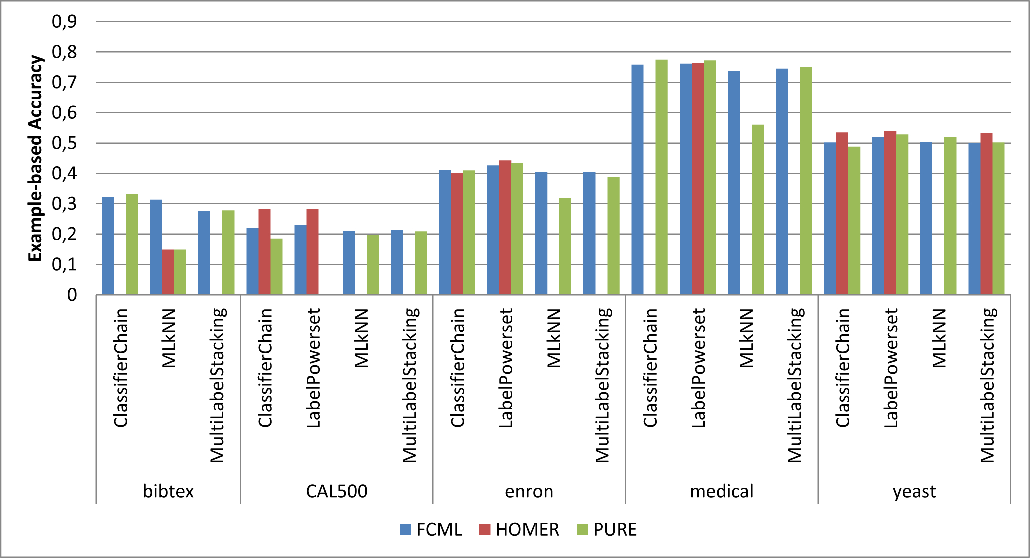
\includegraphics[width=.73\textwidth]{figures/fcml_acc.pdf}
				}
				\subfigure[Micro-averaged F-Measure]{
					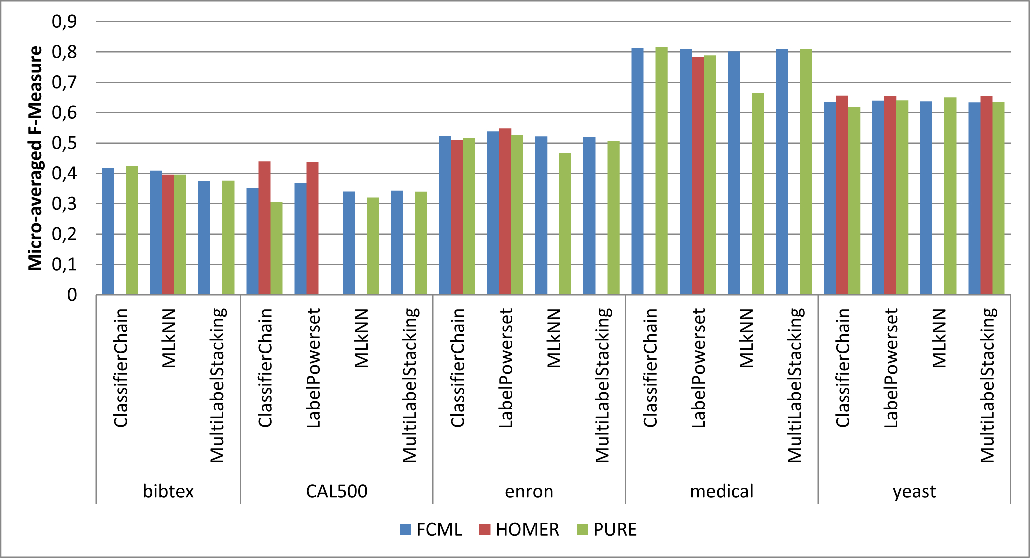
\includegraphics[width=.73\textwidth]{figures/fcml_fmeasure.pdf}
				}
				\subfigure[Hamming Loss]{
					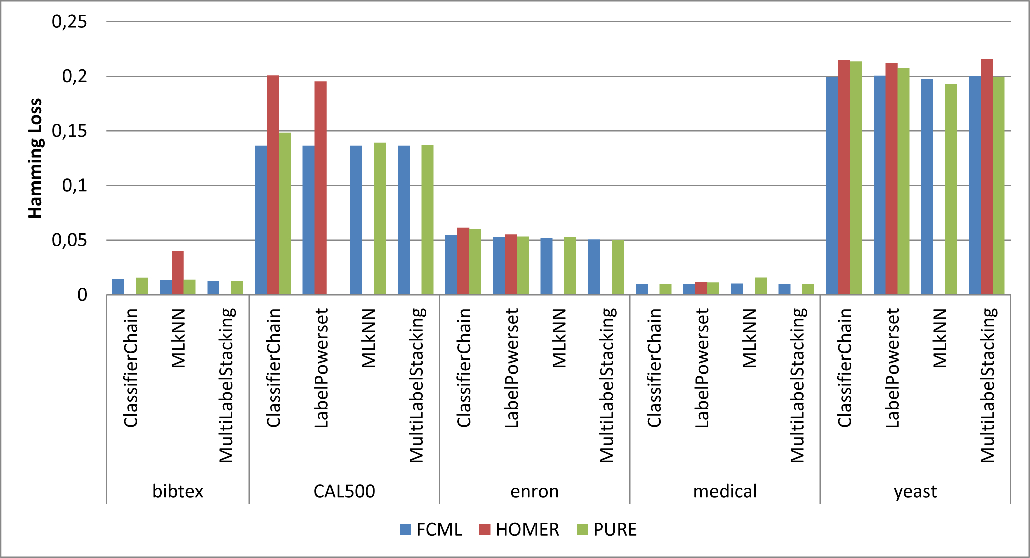
\includegraphics[width=.73\textwidth]{figures/fcml_hamming.pdf}
				}
				\caption{FCML compared to pure multi-label learners and HOMER on different datasets. In every setting the best result is presented. HOMER did not finish on all scenarios.}
				\label{fig:fcml_res}
			\end{figure}

			FCML does not show superior results in Example-based Accuracy. Merely Hamming Loss could be reduced in some cases. Still, ML-kNN could be enhanced in some cases: \textit{enron}, \textit{medical}, \textit{bibtex}. HOMER performs better in almost any case. Best results for FCML in this scenario are achieved with $nc=158$ being a clustering of every label into a sole cluster which indicates there are very few dependencies in the label space.

			In terms of Hamming Loss or Micro-Averaged F-Measure, FCML can achieve small enhancements to the pure and HOMER multi-label learner. Both Hamming Loss and Micro-Averaged F-Measure take false positives into account, while accuracy does not. That indicates that FCML has slightly better performance in predicting absent labels compared to pure and HOMER. By reducing the label space and therefore reducing the influences of other labels, non-relevant and misleading signals are eliminated.

			It is problem to identify the effect of $nc$ on the performance as different multi-label learners perform best on very different $nc$: For example the \textit{bibtext} dataset with $|L|=158$, where Classifier Chains have the best result with a $nc=8$, MlKNN $k=158$ and MultiLabel-Stacking with $nc=14$.

			\subsubsection{Summary}

				The results show that a clustering of labels into different groups and splitting the dataset according to those label sets does not cause a lower predicting performance. Even very strong splitting, where every label falls into a single cluster, may enhance the performance, what indicates that inter-label relations are not used. Prediction of absent labels could be slightly enhanced, indicated by lower Hamming Loss results. This is done by reducing the noise in the label-space by grouping them into smaller subsets.
		
		\chapter{Conclusions}
\label{chapter:Conclusions}

	This work aims to find subgroups of labels and features in multi-label classification. It was expected to gain a significant enhancement of predicting performance. This claim could not be yet verified in its entirety.

	However, results show that a splitting is possible without losing label information. Also small improvements in predicting true negative labels could be shown. Label dependencies in multi-label problems are still under research. Current work \cite{cheng10icmlmld} shows that label dependencies may have to be considered in even more detail than done so far.

	For identifying label groups, clustering methods are used. To enhance the clustering, feature selection algorithms have been applied, increasing the focus on attribute relations. For this, different cluster and feature-selection methods were evaluated. A framework for group-based multi-label classification has been implemented using the MULAN Java Library.

	The idea of this work suffered from the complexity of its components, clustering and feature selection. Future work must aim to analyze the effects of the numerous parameters in more detail, than it could be done in the limited time of the bachelor thesis. Finding the ideal number of clusters is still subject of research in the field of unsupervised clustering. For example, the datasets could be evaluated in terms of density, label distribution and label correlation. Also, it would be a  beneficial to find a rule to specify the number of clusters $nc$ dependent to the label space. In addition, the feature selection process could be evaluated in more detail.

	Also, it seems to be promising to develop some horizontal splitting, where groups are not only subsets of attributes but also subsets of instances with high specificity to certain label (sub)sets. New bi-clustering algorithms seem to be a suitable solution for this task.

	In conclusion, first steps towards for Label- and Feature-Selection in Multi-Label Classification were taken. Due to time limitations not all aspects of involved methods could yet be treated in full detail, which may achieve improved performance. However, this work may serve as a starting point to future work in Label and Feature Selection in Multi-Label Classification.
%		
%		\addcontentsline{toc}{part}{Appendix}
%		
%		\appendix %---------------------------------------
%		
%		\chapter{Detailed Descriptions}
%\section{Detailed Validation Results}
\label{chapter:DetailedDescriptions}
Here come the details that are not supposed to be in the regular text.


  	\clearemptydoublepage
  
	\bibliography{bibliography/literature}
	
 
\end{document}

